\chapter{ЭКСПЕРИМЕНТАЛЬНОЕ ИССЛЕДОВАНИЕ ПНЕВМОПРИВОДА С ДИСКРЕТНЫМ УПРАВЛЕНИЕМ}\label{ch:ch4}
Основная цель данной части работы заключается в проверке разработанных
математических моделей и алгоритмов управления,
а также экспериментальном подтверждении их эффективности. Проведение экспериментов позволяет
выявить особенности работы пневмопривода, определить степень влияния
нелинейных факторов на динамику системы и предложить рекомендации по
выбору оптимальных параметров управления для различных условий эксплуатации.

Исследование проводилось на экспериментальной установке,
специально спроектированной для анализа динамических характеристик и
точности позиционирования привода. В данной главе описывается конструкция
установки, включая аппаратную часть и программное обеспечение, детализируется
методика проведения экспериментов и приводятся результаты сравнительного
анализа различных алгоритмов управления. Полученные данные сопоставляются с
теоретическими расчетами, что позволяет оценить точность предложенных моделей
и научно обосновать выбор наиболее эффективных методов управления.

\textbf{Описание экспериментальной установки.}
Экспериментальная установка, разработанная для исследования пневматического привода с
дискретным управлением, представляет собой комплекс технических средств и
программных решений, обеспечивающих проведение экспериментов с достаточной точностью и достоверностью.
Спроектированная установка позволяет реализовать все возможные режимы работы
пневмопривода, включая разгон, торможение и удержание,
проводить сравнительный анализ эффективности алгоритмов управления.

Экспериментальная установка включает в себя два основных компонента:
аппаратную часть, отвечающую за физическое выполнение процессов управления и
измерение параметров системы, и программное обеспечение, которое реализует
управление приводом, сбор данных и их анализ.

\textbf{Аппаратная часть установки.}
Экспериментальный стенд для исследования алгоритмов управления позиционным пневмоприводом
спроектирован с учетом требований к жесткости конструкции, точности измерений и возможности
варьирования инерционной нагрузки. Основу механической части стенда составляет алюминиевый
конструкционный профиль, обеспечивающий необходимую жесткость и точность базирования компонентов.

На рисунке \ref{fig:experimental_stand} представлена конструкция собранного стенда.
На профиле 1 установлен пневматический цилиндр двустороннего действия, шток которого механически связан
с подвижной платформой 2. Платформа, изготовленная методом трехмерной печати из полимерного материала
(как и остальные опорные элементы и детали),
перемещается по направляющим конструкционного профиля посредством линейных подшипников качения. Данное
техническое решение обеспечивает минимизацию сил трения при движении и высокую точность линейного перемещения.
Конструкция платформы предусматривает возможность установки дополнительных грузов, что позволяет проводить
исследования при различных значениях инерционной нагрузки.
Основные технические характеристики элементов экспериментального стенда представлены в таблице~\ref{tab:stand_parameters},
а полный перечень используемых компонентов приведен в приложении~\ref{app:equipment_list}.

\begin{figure}[ht]
	\centering
	\includegraphics{part4/стенд.pdf}
	\caption{Конструкция экспериментального стенда:\\1 -- алюминиевый профиль;
		2 -- пневмоцилиндр; 3 -- подвижная платформа; 4 -- дискретные распределители;
		5 -- датчики давления; 6 -- потенциометрический датчик}
	\label{fig:experimental_stand}
\end{figure}

\begin{table}[h]
	\centering
	\caption{Расширенные параметры моделирования электропневматического привода}
	\small
	\begin{tabular}{lll}
		\textbf{Параметр} & \textbf{Значение} & \textbf{Размерность} \\
		\midrule
		Масса платформы   & \num{1.0}         & кг                   \\
		Масса груза       & \num{0.5}         & кг                   \\
		Ход поршня        & \num{0.3}         & м                    \\
		Диаметр поршня    & \num{0.032}       & м                    \\
		Диаметр штока     & \num{0.012}       & м                    \\
		\midrule
	\end{tabular}
	\label{tab:stand_parameters}
\end{table}


Пневматическая часть стенда включает четыре дискретных распределителя с электромагнитным
управлением Camozzi AA31-0C2. Распределители соединены с полостями пневмоцилиндра посредством пневматических линий.
Для контроля термодинамических процессов в полостях пневмоцилиндра установлены два датчика давления Festo SPAU-P10R-H-G18FD-L-PNLK-PNVBA-M8U,
позволяющие измерять текущие значения давлений в поршневой и штоковой полостях. Измерение положения
штока осуществляется прецизионным потенциометрическим датчиком линейного перемещения Festo MLO-POT-450-TLF.

Разработанная конструкция стенда обеспечивает прямолинейность перемещения подвижной части,
минимизацию паразитных нагрузок на шток пневмоцилиндра, возможность варьирования массы подвижной
части и удобство монтажа измерительной аппаратуры. Наличие датчиков давления в полостях пневмоцилиндра
в сочетании с прецизионным измерением положения позволяет получать полную информацию о динамическом
состоянии системы, необходимую для исследования эффективности различных алгоритмов управления.
% На рисунке \ref{fig:experimental_setup} представлена схема экспериментальной установки.


Система управления экспериментального стенда реализована по иерархическому принципу и включает три
основных уровня: исполнительный уровень, уровень управления реального времени и уровень человеко-машинного интерфейса.
Структурная схема системы представлена на рисунке \ref{fig:control_system_diagram}.

\begin{figure}[ht]
	\centering
	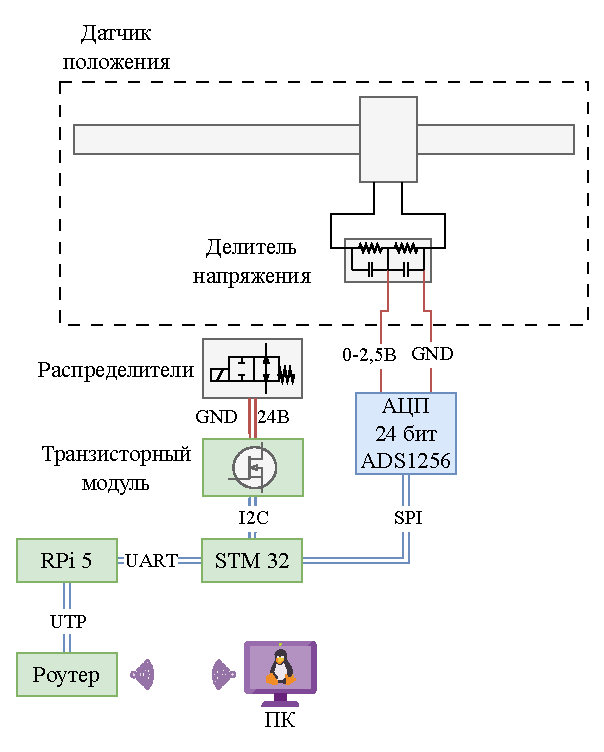
\includegraphics{part5/стурктурная диаграма су.pdf}
	\caption{Структурная схема системы управления экспериментальным стендом}
	\label{fig:control_system_diagram}
\end{figure}

Исполнительный уровень системы объединяет датчики и актуаторы стенда. В его состав входит
24-битный аналого-цифровой преобразователь, осуществляющий измерение положения штока пневмоцилиндра,
а также силовой модуль на полевых транзисторах, обеспечивающий коммутацию четырех дискретных
распределителей.

Центральным элементом уровня управления реального времени является микроконтроллер
STM32 NUCLEO-F767ZI. Данный контроллер осуществляет сбор данных с АЦП по интерфейсу SPI с частотой дискретизации
1 кГц, реализует алгоритмы управления в реальном времени и формирует управляющие воздействия на
распределители через MOSFET-модуль. Обмен данными с верхним уровнем системы производится по
интерфейсу UART. В процессе работы микроконтроллер принимает от верхнего уровня целевое положение
штока пневмоцилиндра, коэффициенты настройки алгоритма управления, максимальное время выполнения
управления, а также команды запуска и останова процесса управления. В режиме реального времени
осуществляется передача телеметрической информации, содержащей текущее положение штока,
оценку скорости движения, состояния распределителей и время с начала процесса управления.

Верхний уровень системы реализован на базе одноплатного компьютера Raspberry Pi 5,
который выполняет функции веб-сервера для обеспечения пользовательского интерфейса
На данном уровне производится обработка команд пользователя, визуализация процесса
управления в реальном времени, расчет показателей качества управления и архивирование
экспериментальных данных. Взаимодействие пользователя с системой осуществляется через веб-интерфейс,
позволяющий задавать параметры эксперимента, осуществлять управление процессом, наблюдать
текущие данные в виде графиков и производить анализ результатов экспериментов.

Разработанная архитектура системы управления обеспечивает высокую точность измерений благодаря
применению прецизионного АЦП, гарантированное время реакции системы за счет реализации
алгоритмов управления на микроконтроллере, удобство проведения экспериментов
через веб-интерфейс и возможность детального анализа результатов испытаний.

\textbf{Программное обеспечение установки.}
Программное обеспечение установки, как описано ранее, построено на основе клиент-серверной архитектуры,
где серверная часть реализована на одноплатном компьютере (Raspberry Pi 5), а периферийное
управление осуществляется посредством микроконтроллера STM32. Такое разделение позволяет
распределить задачи между вычислительными узлами: Raspberry Pi обеспечивает высокоуровневую
обработку данных, реализацию веб-интерфейса и взаимодействие с базой данных, в то время как
STM32 отвечает за реализацию алгоритмов управления в реальном времени и непосредственное
взаимодействие с исполнительными механизмами.

Программное обеспечение установки разделено на несколько основных модулей:

\textbf{Модуль веб-интерфейса и пользовательского взаимодействия.} Данный модуль реализует графический интерфейс для оператора
установки, позволяющий выбирать режим эксперимента (одиночный или множественный), настраивать алгоритмы управления,
вводить параметры и просматривать результаты эксперимента в виде графиков и таблиц.
Интерфейс представлен на рисунке \ref{fig:web_interface}.

\begin{figure}[ht]
	\centering
	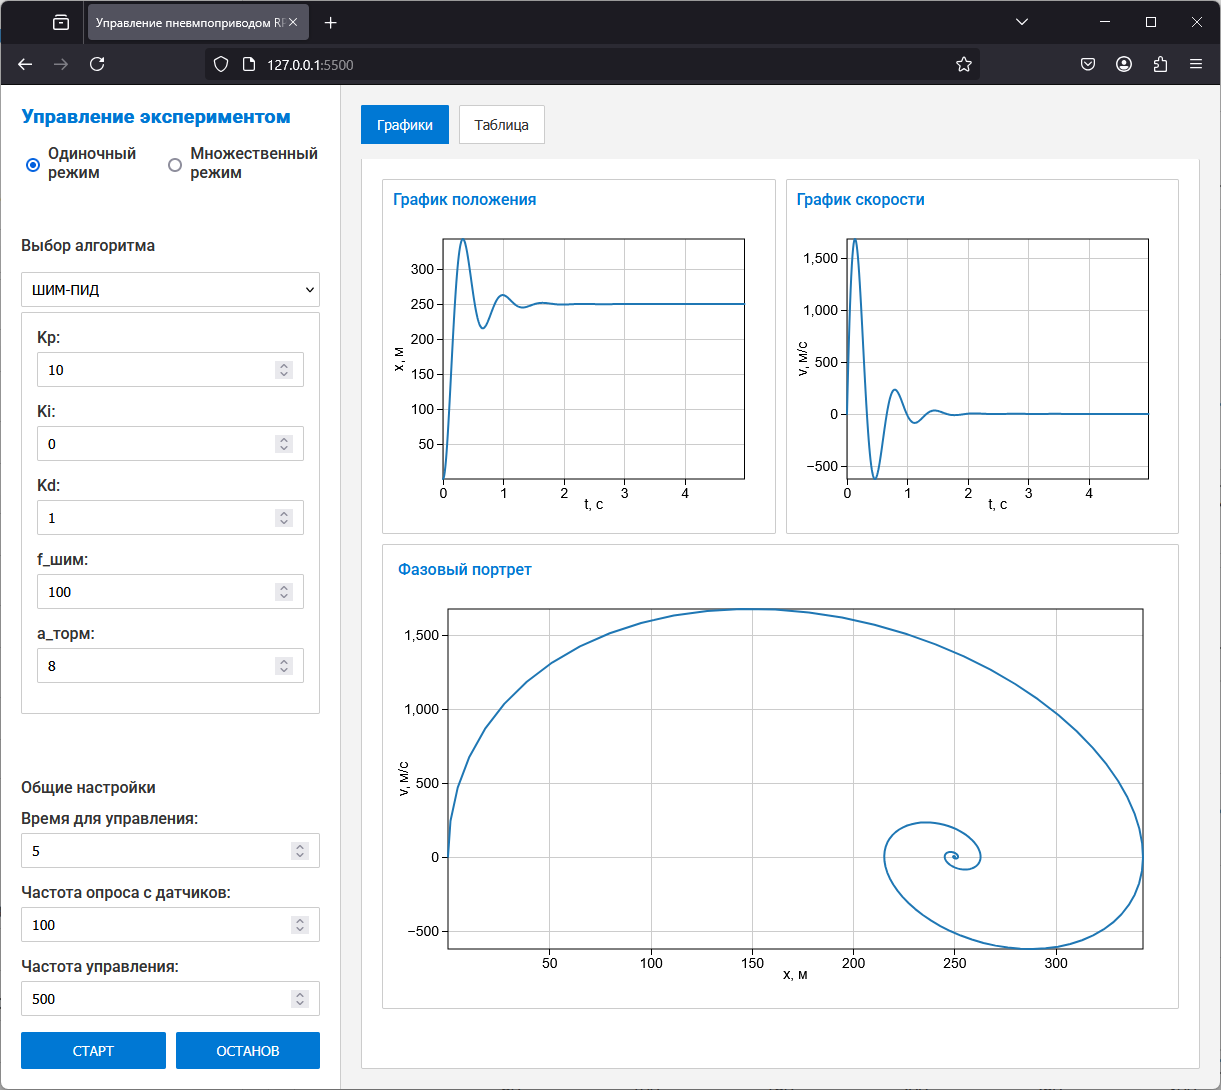
\includegraphics[width=0.8\textwidth]{part5/Снимок экрана 2025-02-27 144410.png}
	\caption{Веб-интерфейс системы управления}
	\label{fig:web_interface}
\end{figure}

\textbf{Модуль управления экспериментом.} Основная логика управления экспериментом реализована на стороне сервера
(Raspberry Pi). Модуль обеспечивает сбор параметров, введённых оператором, их валидацию и передачу на микроконтроллер STM32.
В данном модуле также реализованы алгоритмы синхронизации, обработка данных с STM32 и логирование
ключевых событий эксперимента.

\textbf{Модуль управления исполнительными механизмами.} Данный модуль реализован на микроконтроллере STM32 и
представляет из себя отдельное программное обеспечение, обеспечивающее управление дискретными распределителями,
опрос датчиков, реализацию всех алгоритмов управления и обмен данными с Raspberry Pi по интерфейсу UART.

\section{Постановка задач и программы экспериментального исследования позиционирования пневмопривода}
Основной целью экспериментального исследования является проверка математических моделей и алгоритмов управления позиционным
пневмоприводом с дискретными распределителями, разработанных в теоретических разделах данной работы,
а также оценка их практической эффективности на реальной физической установке.
Проведение натурных экспериментов направлено на решение следующих ключевых задач:

\begin{enumerate}
	\item \textbf{Экспериментальное определение параметров модели:}
	      провести идентификацию ключевых параметров математической модели,
	      которые сложно или невозможно точно определить теоретически, в частности:

	      \begin{itemize}
		      \item выполнить тарировку потенциометрического датчика положения
		            для обеспечения точных измерений перемещения штока;
		      \item экспериментально измерить силу трения в различных режимах движения
		            (гармонические колебания, разгон/торможение, реверсы) и
		            идентифицировать параметры модели трения LuGre;
		      \item экспериментально определить скорость переключения распределителей
		            и время задержки в системе управления.
	      \end{itemize}
	\item \textbf{Получение и анализ экспериментальных данных о переходных процессах позиционирования:}
	      провести серию экспериментов с различными алгоритмами управления (ПИД-регулятор с ШИМ,
	      управление в скользящих режимах, нечеткое управление, прогнозное управление) для получения данных о переходных процессах
	      позиционирования, провести анализ полученных данных и оценить влияние параметров управления
	      на динамические и ресурсные характеристики системы.

	\item \textbf{Оценка точности математической модели:}
	      оценить адекватность разработанной математической модели путем сопоставления результатов
	      численного моделирования с данными, полученными на экспериментальной установке для
	      различных алгоритмов управления (ПИД с ШИМ, управление в скользящих режимах
	      различных конфигураций, нечеткое управление, прогнозное управление).
\end{enumerate}

Программа экспериментального исследования включает в себя следующие этапы:
\begin{enumerate}
	\item \textbf{Подготовительный этап:} Сборка и наладка экспериментального стенда, проверка работоспособности
	      всех компонентов (пневмоцилиндр, распределители, датчики, система управления), настройка программного обеспечения.
	\item \textbf{Определение параметров модели:}
	      \begin{enumerate}
		      \item тарировка потенциометрического датчика положения;
		      \item измерение силы трения в различных режимах движения (гармонические колебания, разгон/торможение, реверсы);
		      \item идентификация параметров модели трения LuGre;
		      \item измерение времени переключения распределителей и задержки в системе управления.
	      \end{enumerate}
	\item \textbf{Исследование переходных процессов позиционирования:}
	      \begin{enumerate}
		      \item проведение экспериментов с различными алгоритмами управления (ПИД-регулятор с ШИМ,
		            управление в скользящих режимах, нечеткое управление, прогнозное управление);
		      \item сбор и анализ данных о переходных процессах позиционирования.
	      \end{enumerate}
	\item \textbf{Оценка точности математической модели:}
	      \begin{enumerate}
		      \item сравнение результатов численного моделирования с экспериментальными данными;
		      \item оценка адекватности разработанной математической модели.
	      \end{enumerate}
\end{enumerate}

\textbf{Автоматизация процесса экспериментального исследования.}
Ключевой особенностью разработанной экспериментальной установки является высокий уровень автоматизации процесса
исследований, что позволяет проводить масштабные серии экспериментов без постоянного участия оператора.
Автоматизация процесса экспериментального исследования обеспечивается специализированными
алгоритмами, интегрированными в описанное ранее программное обеспечение.

Система поддерживает только полнофакторное исследование, при котором осуществляется систематический перебор
всех комбинаций параметров из заданных диапазонов с фиксированным шагом. Для каждого алгоритма
управления определяются ключевые параметры и границы их изменения. Например, для ПИД-регулятора
с ШИМ исследуются комбинации коэффициентов $K_{\text{п}} \in [1, 30]$, $K_{\text{и}} \in [0, 1]$,
$K_{\text{д}} \in [0, 20]$ с соответствующими шагами дискретизации и частотой ШИМ
$f_{\text{ШИМ}} \in [10, 50]$ Гц.

\textbf{Автоматическое проведение экспериментов.} Для каждой серии экспериментов оператор задаёт
через веб-интерфейс параметры плана исследования:

\begin{itemize}
	\item исследуемые алгоритмы управления и их параметрические конфигурации;
	\item траектории перемещения (последовательность целевых положений);
	\item настройки статистической обработки (количество повторений, доверительные интервалы);
	\item критерии автоматической остановки при выявлении нештатных ситуаций;
	\item режимы паузы между экспериментами для обеспечения идентичных тепловых условий.
\end{itemize}

Система автоматически формирует очередь экспериментов, которые затем выполняются
последовательно без участия человека. Каждый эксперимент включает следующие этапы:

\begin{itemize}
	\item инициализация системы и установка начальных условий;
	\item настройка параметров алгоритма управления согласно плану эксперимента;
	\item выполнение управляющего воздействия и регистрация динамических параметров;
	\item автоматический расчёт показателей качества управления;
	\item сохранение результатов в базе данных с привязкой к параметрам эксперимента;
	\item возврат системы в исходное состояние и подготовка к следующему эксперименту.
\end{itemize}

Система включает встроенные механизмы диагностики, обеспечивающие автоматическое прерывание эксперимента
при обнаружении аномалий (превышение максимальных давлений, нештатная скорость движения, выход за пределы рабочей зоны).

\textbf{Преимущества автоматизированного подхода к исследованиям.} Реализованная система автоматизации обеспечила:
\begin{itemize}
	\item многократное повторение идентичных экспериментов для статистической обработки результатов;
	\item стандартизацию условий проведения экспериментов, что повысило сопоставимость данных, полученных для различных алгоритмов;
	\item возможность исследования сложных многопараметрических зависимостей и оптимизации регуляторов по множеству критериев;
	\item формирование обширной базы экспериментальных данных (более 200 экспериментов) с возможностью их систематизации и многофакторного анализа.
\end{itemize}

Созданная автоматизированная система позволила не только существенно повысить производительность экспериментальных исследований,
но и обеспечить более глубокий анализ характеристик различных алгоритмов управления за счёт получения статистически значимых выборок для каждой исследуемой конфигурации параметров.

Разработанное программное обеспечение реализует следующие функции:
\begin{itemize}
	\item автоматическое последовательное выполнение серий экспериментов с различными алгоритмами управления
	      и их параметрами без вмешательства оператора;
	\item задание многомерной сетки параметров для каждого алгоритма управления и автоматический перебор
	      всех комбинаций значений в соответствии с планом эксперимента;
	\item циклическое повторение каждого эксперимента заданное количество раз для обеспечения
	      статистической достоверности результатов;
	\item автоматическое сохранение и структурирование экспериментальных данных в базе данных с
	      привязкой к параметрам эксперимента;
	\item оперативный расчёт показателей качества управления (время переходного процесса, статическая
	      ошибка, перерегулирование, интегральные критерии) и их автоматическая запись;
	\item непрерывный мониторинг состояния экспериментальной установки с функциями автоматической
	      диагностики и защиты от аварийных ситуаций.
\end{itemize}
Автоматизированный режим позволяет проводить эксперименты в непрерывном режиме без постоянного присутствия
оператора, что существенно повышает производительность исследований. Для каждой серии экспериментов оператор
задаёт через веб-интерфейс план исследования, включающий:
\begin{itemize}
	\item тип алгоритма управления (ПИД с ШИМ, УСР с различными конфигурациями, нечёткое управление,
	      прогнозное управление);
	\item диапазоны изменения параметров алгоритма и шаг дискретизации для каждого параметра;
	\item целевые положения штока и последовательность их изменения;
	\item количество повторений каждого эксперимента;
	\item паузы между экспериментами для стабилизации теплового режима установки.
\end{itemize}

По итогам автоматизированных экспериментальных исследований для каждого алгоритма управления сформирована база данных,
содержащая более 200 экспериментов с различными комбинациями параметров, что обеспечило высокую достоверность
результатов сравнительного анализа и оптимизации алгоритмов управления.

\section{Экспериментальное определение параметров модели}

\textbf{Тарировка потенциометрического датчика положения.}
Для измерения положения штока пневмопривода используется потенциометрический датчик линейных перемещений,
требующий тарировки для преобразования выходного напряжения в единицы длины. В качестве эталонного средства
измерения применялся линейный инкрементальный энкодер с дискретностью 5 мкм. Тарировочные испытания проводились
в статическом режиме для исключения влияния динамических погрешностей.

Измерения выполнялись в контрольных точках с шагом 50 мм по всей длине хода штока пневмопривода (350 мм).
В каждой точке производилась регистрация показаний потенциометра и эталонного энкодера.
Результаты измерений представлены в таблице \ref{tab:calibration_data}.

\begin{table}[ht]
	\centering
	\caption{Результаты тарировочных измерений}\label{tab:calibration_data}
	\small
	\begin{tabular}{lll}
		\hline
		\textbf{Положение}, мм & \textbf{Напряжение}, В & \textbf{СКО напряжения}, В \\
		\hline
		0                      & \num{0.072000}         & $\num{2.54}\cdot 10^{-5}$  \\
		50                     & \num{0.297625}         & $\num{2.58}\cdot 10^{-5}$  \\
		100                    & \num{0.523250}         & $\num{2.62}\cdot 10^{-5}$  \\
		150                    & \num{0.748875}         & $\num{2.57}\cdot 10^{-5}$  \\
		200                    & \num{0.974500}         & $\num{2.59}\cdot 10^{-5}$  \\
		250                    & \num{1.200125}         & $\num{2.60}\cdot 10^{-5}$  \\
		300                    & \num{1.425750}         & $\num{2.58}\cdot 10^{-5}$  \\
		350                    & \num{1.647625}         & $\num{2.61}\cdot 10^{-5}$  \\
		\hline
	\end{tabular}
\end{table}

Для оценки стабильности показаний датчика проведен анализ серии измерений в крайнем положении штока
(350 мм). Зарегистрированные значения напряжения находились в диапазоне от \num{1.647577}~В до \num{1.647685} В,
что соответствует среднеквадратическому отклонению $\sigma_U = \num{2.61} \cdot 10^{-5}$ В.

На основе полученных данных методом наименьших квадратов построена
тарировочная характеристика. Зависимость перемещения от напряжения аппроксимировалась линейной функцией:
\begin{equation}
	x = \num{222.15}U - \num{16.00},
\end{equation}
где $x$ -- перемещение в миллиметрах, $U$ -- напряжение в вольтах.

Тарировочная характеристика представлена на рисунке \ref{fig:calibration}.
Анализ остатков (разностей между экспериментальными и расчетными значениями) показывает их
случайный характер без выраженных систематических составляющих. Среднеквадратическое отклонение остатков
составляет \num{0.042}~мм, а максимальная абсолютная погрешность не превышает \num{0.087}~мм. Высокое значение
коэффициента детерминации $R^2 = \num{0.9998}$ подтверждает линейность характеристики датчика во всем диапазоне измерений.


\begin{figure}[ht]
	\centering
	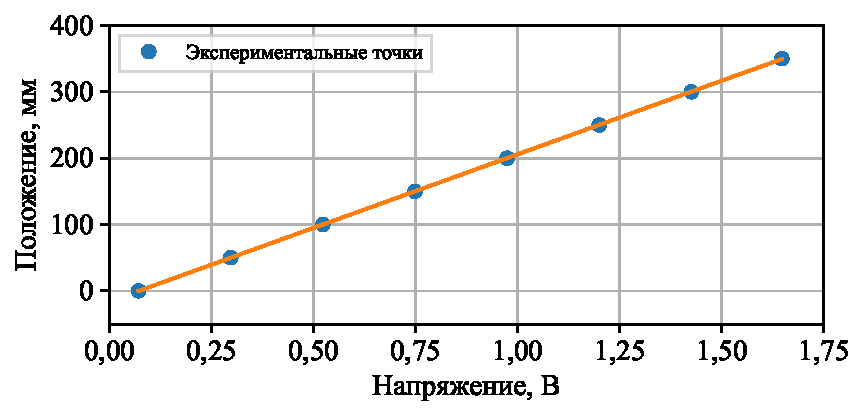
\includegraphics{part5/calibration_curve.pdf}
	\caption{Тарировочная характеристика потенциометрического датчика}\label{fig:calibration}
\end{figure}

Флуктуации напряжения вносят пренебрежимо малый вклад в общую погрешность измерения положения штока.
Максимальное отклонение положения, вызванное нестабильностью напряжения, не превышает 24 мкм, что
существенно меньше требуемой точности позиционирования пневмопривода. Для дополнительного снижения
влияния случайных выбросов напряжения реализована программная фильтрация сигнала методом экспоненциального сглаживания:

\begin{equation}
	U_t = \alpha U_{изм} + (1-\alpha)U_{t-1},
\end{equation}
где $U_t$ -- сглаженное значение напряжения;
$U_{изм}$ -- текущее измеренное значение;
$U_{t-1}$ -- предыдущее сглаженное значение;
$\alpha$ -- коэффициент сглаживания ($\alpha = \num{0.2}$).

Применение экспоненциального фильтра позволяет снизить среднеквадратическое отклонение измеряемого напряжения до $\num{1.2} \cdot 10^{-5}$ В без
внесения существенной динамической погрешности в процессе движения штока. Сравнение исходного и сглаженного сигналов представлено на рисунке \ref{fig:voltage_filtering}.
\begin{figure}[ht]
	\centering
	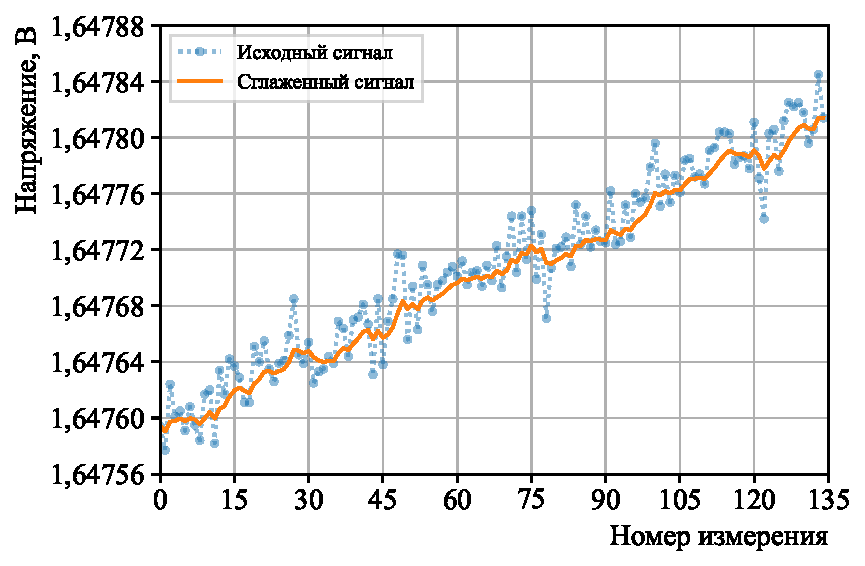
\includegraphics{part5/voltage_filtering.pdf}
	\caption{Сравнение исходного и сглаженного сигналов датчика}\label{fig:voltage_filtering}
\end{figure}

\textbf{Экспериментальное измерение силы трения.}
Дальнейшим этапом является экспериментальное определение силы трения, возникающей при движении платформы
пневматическим приводом вдоль линейных направляющих, а также последующая идентификация
параметров параметров модели LuGre на основе полученных данных.

Для точного измерения силы трения необходимо собрать качественные экспериментальные данные
при различных режимах движения платформы. Эксперименты проводились в следующих режимах:

\begin{enumerate}
	\item Гармонические колебания: платформа приводилась в синусоидальные колебания
	      с различными амплитудами и частотами, чтобы оценить поведение трения в динамических условиях.

	\item Постепенный разгон и торможение: платформа разгонялась до заданной скорости,
	      удерживалась на постоянной скорости, а затем плавно тормозилась до
	      полной остановки. Это позволило изучить переходные процессы и устойчивость системы.

	\item Многократные реверсы движения: повторялись циклы движения платформы вперед и
	      назад для выявления эффектов гистерезиса и асимметрии трения при смене направления движения.
\end{enumerate}

Каждый режим движения выполнялся по $n = 5$ раз для обеспечения статистической
достоверности результатов и оценки вариабельности измерений.

В ходе каждого эксперимента регистрировались следующие сигналы:
\begin{itemize}
	\item давления в полостях цилиндра $p_1(t), p_2(t)$, измеряемые с частотой $f_s = 100$ Гц;
	\item положение платформы $x(t)$, измеряемое с частотой $f_s = 100$ Гц и разрешением $d_x = 0.01$ мм;
	\item ускорение $\ddot{x}(t)$ платформы, измеряемое датчиком ускорения с частотой $f_s = 100$ Гц;
	\item скорость $\dot{x}(t)$ платформы, вычисляемая по данным датчика положения с применением фильтра
	      низких частот (фильтр Баттерворта 4-го порядка с частотой среза $f_\text{с} = 50$~Гц) для уменьшения шума.
\end{itemize}

Все сырые данные подвергались предварительной обработке, включающей фильтрацию для устранения высокочастотных помех
и калибровку датчиков. Примерно обработанные сигналы представлены на рисунке \ref{fig:raw_data}.

\begin{figure}[ht]
	\centering
	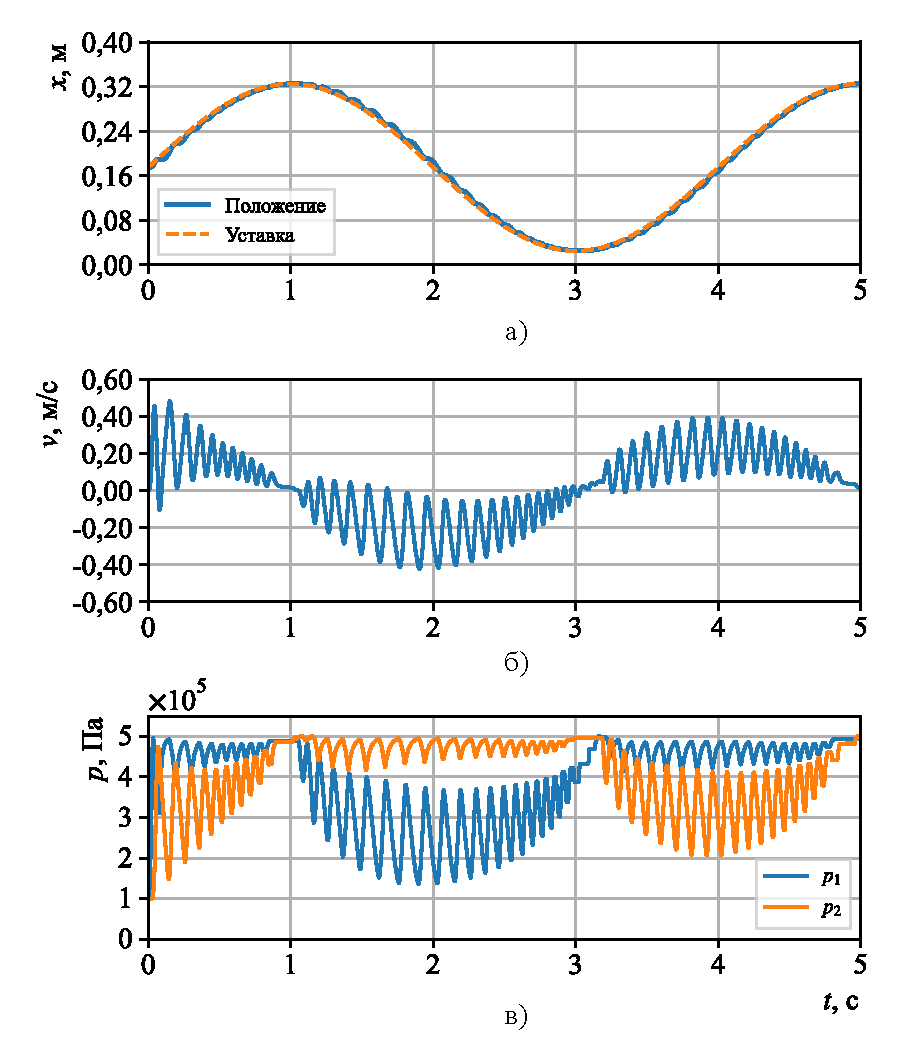
\includegraphics{part5/harmonic_real_f0.25_a0.15.pdf}
	\caption{Пример обработанных данных эксперимента}\label{fig:raw_data}
\end{figure}

На основе записанных данных сила пневмоцилиндра рассчитывалась по формуле:

\begin{equation}
	R_\text{пнев}(t) = F_1 p_1(t) - F_2 p_2(t).
\end{equation}

Затем, используя второй закон Ньютона, экспериментальная сила трения определялась как:

\begin{equation}
	R_\text{тр, эксп}(t) = R_\text{пнев}(t) - M \ddot{x}(t).
\end{equation}
При условии горизонтального расположения стенда и отсутствия дополнительных сил $R_\text{доп} \approx 0$.
Для описания динамики трения использовалась модель LuGre, представленная выражениями \ref{eq:ch2/lugre},
а параметры модели $\theta = \{f_c, f_s, n, \sigma_0, \sigma_1, \sigma_2\}$ определялись путем минимизации ошибки
методом наименьших квадратов:

\begin{equation}
	J(\theta) = \sum_{i=1}^N \left[ R_\text{тр, эксп}(t_i) - R_\text{тр, мод}(t_i, \theta) \right]^2.
\end{equation}

Для решения этой задачи использовался алгоритм Левенберга-Марквардта.
На каждом шаге итерации для заданного набора параметров $\theta$ численно интегрировались уравнения модели
трения, после чего рассчитывалась теоретическая сила $R_\text{тр, мод}(t)$. Разница
между экспериментальными и модельными значениями суммировалась
в функцию ошибки, которая минимизировалась до сходимости алгоритма. Полученные параметры модели
представлены в таблице \ref{tab:lugre_params}.

\begin{table}[ht]
	\caption{Параметры модели трения LuGre}
	\label{tab:lugre_params}
	\centering
	\small
	\begin{tabular}{lll}
		\hline
		\textbf{Параметр} & \textbf{Значение} & \textbf{Единица измерения}    \\
		\hline
		$f_c$             & \num{35.0718}     & Н                             \\
		$f_s$             & \num{47.1895}     & Н                             \\
		$v_s$             & \num{0.0151}      & \si{\metre\per\second}        \\
		$\sigma_0$        & \num{14280.0364}  & \si{\newton\per\metre}        \\
		$\sigma_1$        & \num{2.0924d-25}  & \si{\newton\second\per\metre} \\
		$\sigma_2$        & \num{385.4551}    & \si{\newton\second\per\metre} \\
		\hline
	\end{tabular}
\end{table}

На рисунке \ref{fig:friction_force} представлены результаты экспериментального измерения силы трения и ее модельное
представление на основе параметров LuGre. Видно, что модель хорошо описывает динамику трения во всем диапазоне
измерений, включая переходные процессы и реверсы движения.

\begin{figure}[ht]
	\centering
	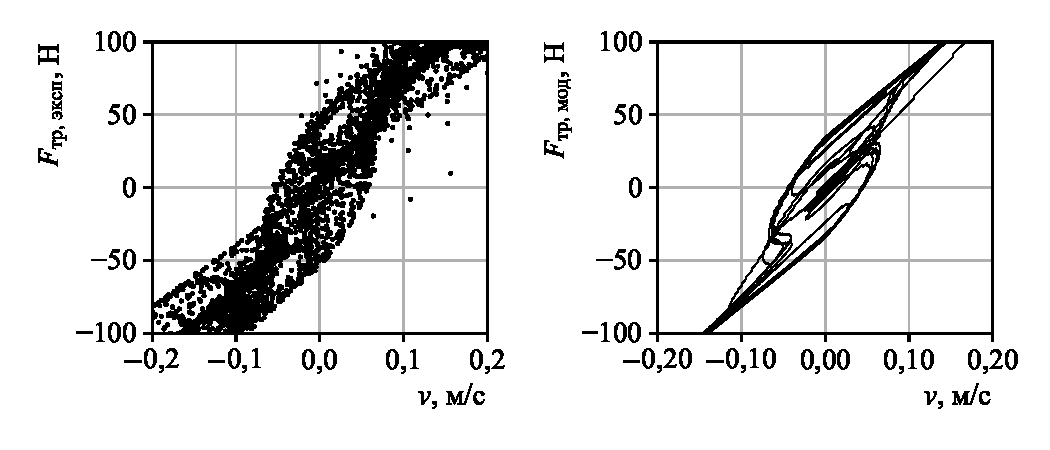
\includegraphics{part4/friction_experiment_fv.pdf}
	\caption{Сравнение экспериментальной и модельной силы трения}\label{fig:friction_force}
\end{figure}

Для количественной оценки качества соответствия модели и экспериментальных данных был рассчитан коэффициент детерминации
$R^2$, который составил \num{0.98229}, указывая на высокую степень согласованности. Среднеквадратичная ошибка составила
\num{11.4002}~\si{\newton}, что соответствует \num{5.7}\% от средних значений сил трения, наблюдаемых в системе.

\textbf{Экспериментальное измерение времени переключения распределителей.}
Динамические характеристики дискретных распределителей оказывают существенное влияние на быстродействие
и точность позиционирования пневмопривода. Для корректного моделирования переходных процессов в
системе необходимо экспериментально определить время срабатывания и динамику переключения распределителей.

Для экспериментального определения времени срабатывания дискретных распределителей использовалась следующая методика.
Распределитель подключался к пневматической магистрали с давлением 5 бар на входе,
а его выход соединялся с с пневмоцилиндром с жестко зафиксированным штоком на расстоянии $x=\num{0.1}\text{м}$.
При подаче электрического управляющего сигнала на электромагнит распределителя
фиксировались изменения давления в измерительной камере и ток в цепи электромагнита.

Временные параметры срабатывания распределителя определялись на основе анализа переходных процессов изменения
давления в измерительной камере и тока в цепи электромагнита. Важно отметить, что процесс открытия
распределителя имеет непрерывный характер, при котором по мере нарастания тока в соленоиде начинается
движение запорно-регулирующего элемента, постепенно увеличивающее проходное сечение. Это приводит к плавному
нарастанию давления в измерительной камере, синхронизированному с перемещением соленоида.

В процессе эксперимента регистрировались следующие основные временные параметры:
\begin{enumerate}
	\item \textbf{Время нарастания тока} $t_{\text{нар}}$ -- интервал времени от
	      начала нарастания тока до достижения 95\% от установившегося значения.

	\item \textbf{Время нарастания давления} $t_{\text{дав}}$ -- интервал времени от
	      начала изменения давления до достижения давлением 95\% от установившегося значения.
	      Этот интервал соответствует процессу перемещения запорно-регулирующего элемента от начала движения до положения, близкого к полному открытию.

\end{enumerate}

Эксперименты проводились для процессов открытия и закрытия распределителя. Для каждого распределителя
выполнялось не менее 10 повторных измерений для обеспечения статистической достоверности результатов.

На рисунке~\ref{fig} представлены типичные осциллограммы переходных процессов при срабатывании распределителя Camozzi A331-0C2.
\begin{figure}[ht]
	\centering
	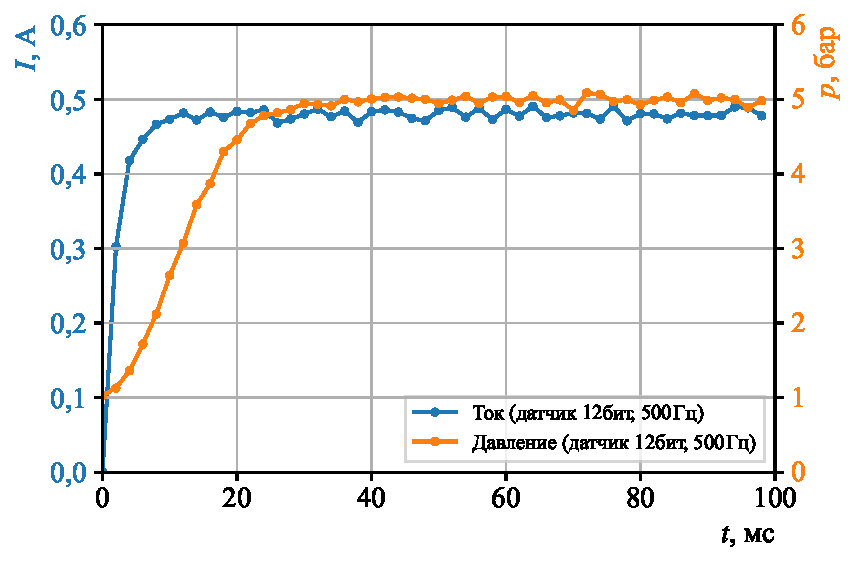
\includegraphics{part4/valve_oscillogramm.pdf}
	\caption{Осциллограммы переходных процессов при срабатывании распределителя}
	\label{fig}
\end{figure}

Анализ полученных осциллограмм позволил определить временные параметры
срабатывания распределителей, которые представлены в таблице~\ref{tab_camozzi}.
\begin{table}[ht]
	\centering
	\caption{Временные параметры срабатывания распределителей Camozzi A331-0C2}
	\label{tab_camozzi}
	\small
	\begin{tabular}{lccc}
		\midrule
		\textbf{Параметр}                              & \textbf{Открытие} & \textbf{Закрытие} & \textbf{СКО} \\
		\midrule
		Время нарастания тока $t_{\text{нар}}$, мс     & \num{9.2 }        & \num{6.8 }        & \num{1.1}    \\
		Время нарастания давления $t_{\text{дав}}$, мс & \num{31.2 }       & \num{26.3}        & \num{1.5}    \\
		\midrule
	\end{tabular}
\end{table}

Как видно из таблицы, общее время срабатывания распределителя составляет примерно 31 мс
как при открытии, так и при закрытии. При этом наблюдается различие в структуре
временных составляющих для процессов открытия и закрытия. При открытии распределителя
время нарастания тока больше, чем при закрытии, что связано с индуктивностью катушки соленоида,
а время нарастания давления, напротив, при закрытии больше, что обусловлено характеристиками возвратной пружины.

Стандартное квадратичное отклонение (СКО) общего времени
срабатывания составляет 2,1 мс, что свидетельствует о достаточно высокой повторяемости
динамических характеристик распределителей. Частичное перекрытие во времени
процессов изменения тока и давления подтверждает непрерывный характер открытия
распределителя, при котором нарастание давления начинается еще до достижения током своего установившегося значения.


\section{Экспериментальное исследование переходных процессов при позиционировании}

В данном разделе представлены результаты экспериментального исследования переходных
процессов при позиционировании пневмопривода с дискретными распределителями с
использованием различных алгоритмов управления и их параметров.

Экспериментальные исследования проводились при перемещении штока из начального положения (0 мм)
в целевое положение 200 мм. Для каждого алгоритма управления исследовались переходные процессы
при различных настройках регулятора.

Для каждого эксперимента регистрировались следующие параметры:
\begin{itemize}
	\item перемещение штока пневмоцилиндра $x(t)$;
	\item скорость движения $\dot{x}(t)$;
	\item давления в полостях пневмоцилиндра $p_1(t)$ и $p_2(t)$;
	\item комбинации состояний распределителей $\mathbf{u}(t)$;
	\item время переходного процесса $t_{\text{п}}$;
	\item статическая ошибка позиционирования $\Delta_{\text{ст}} = |x_{\text{уст}} - x_{\text{зад}}|$;
	\item перерегулирование $\sigma = \frac{x_{\text{макс}} - x_{\text{зад}}}{x_{\text{зад}}} \cdot 100\%$;
	\item интегральный критерий качества ITAE = $\int_{0}^{T} t|e(t)|dt$;
	\item количество переключений между режимами $N_{\text{п}}$.
\end{itemize}

Под переключением между режимами понимается изменение комбинации
состояний распределителей, например, переход от режима $[0;0;0;0]$ к режиму $[1;0;0;1]$ считается как одно переключение.

\textbf{Исследование переходных процессов пневмопривода с ПИД-регулятором и ШИМ.}
Для ПИД-регулятора с ШИМ исследовались переходные процессы при различных значениях
коэффициентов пропорциональной ($K_{\text{п}}$), интегральной ($K_{\text{и}}$) и дифференциальной ($K_{\text{д}}$) составляющих.
На рисунке~\ref{fig:transient_exp_pid} представлены типичные переходные процессы при различных настройках регулятора.

\begin{figure}[h]
	\centering
	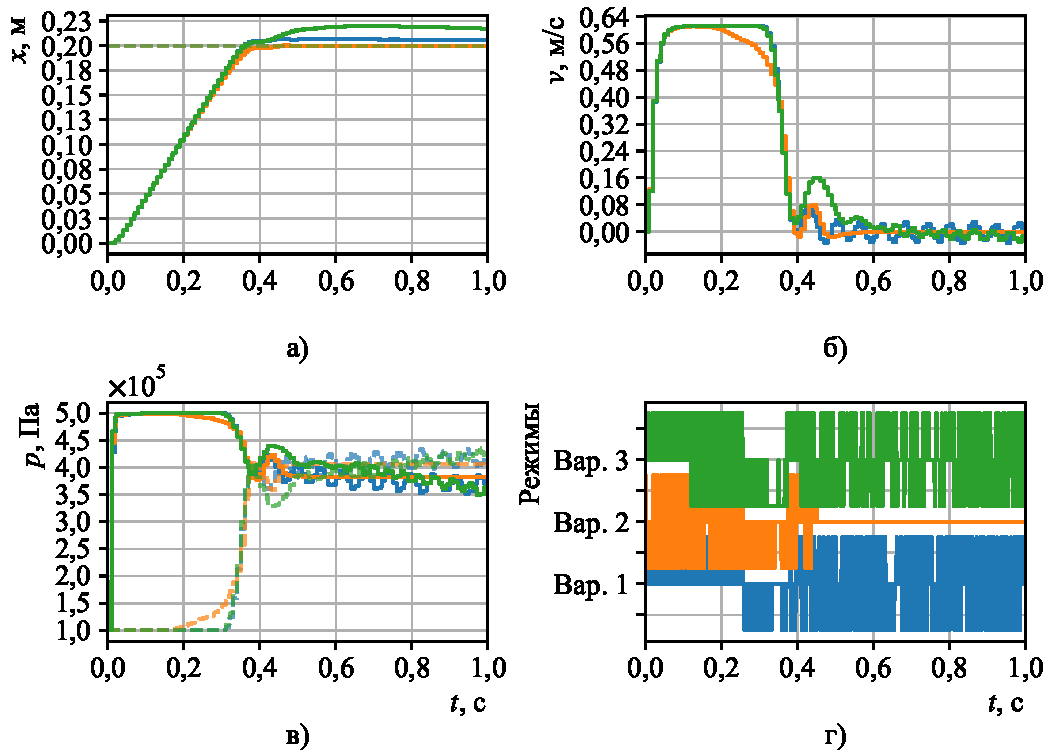
\includegraphics{part4/illust_exp/pid.pdf}
	\caption{Переходные процессы позиционирования с ПИД-регулятором и ШИМ при различных настройках:\\
		а) перемещение штока; б) скорость движения, в) давление в полостях цилиндра; г) комбинация состояний распределителей}
	\label{fig:transient_exp_pid}
\end{figure}

На представленном рисунке \ref{fig:transient_exp_pid} использовались следующие настройки регулятора:
\begin{itemize}
	\item вариант 1: $K_{\text{п}} = 10$, $K_{\text{и}} = 1$, $K_{\text{д}} = 1$;
	\item вариант 2: $K_{\text{п}} = 20$, $K_{\text{и}} = 1$, $K_{\text{д}} = 10$;
	\item вариант 3: $K_{\text{п}} = 30$, $K_{\text{и}} = 1$, $K_{\text{д}} = 20$.
\end{itemize}
Для всех вариантов частота ШИМ-сигнала была установлена равной 10 Гц.

Проведенные испытания позволили определить
ключевые характеристики различных вариантов реализации системы
управления, представленные в таблице~\ref{tab:transition_processes_pid}.

\begin{table}[h]
	\centering
	\caption{Характеристики переходных процессов при различных алгоритмах управления}
	\label{tab:transition_processes_pid}
	\small
	\begin{tabular}{lccc}
		\midrule
		\textbf{Параметр}             & \textbf{Вариант 1} & \textbf{Вариант 2} & \textbf{Вариант 3} \\
		\midrule
		Количество переключений       & 412                & 272                & 527                \\
		Точность позиционирования, мм & 5,74               & 0,60               & 17,01              \\
		Время установления, с         & $\infty$           & 0,37               & $\infty$           \\
		\midrule
	\end{tabular}
\end{table}

Анализ экспериментальных данных позволяет
сделать следующие выводы:

\begin{enumerate}
	\item Вариант 2 демонстрирует существенно лучшие показатели по всем основным критериям:
	      \begin{itemize}
		      \item наименьшее число переключений между режимами (272), что обеспечивает увеличение ресурса системы;
		      \item наивысшую точность позиционирования (0,60 мм);
		      \item конечное время установления (0,37 с).
	      \end{itemize}

	\item Варианты 1 и 3 характеризуются неустойчивым характером переходного процесса
	      (время установления $t_{уст} = \infty$), что указывает на наличие незатухающих колебаний или дрейфа выходного звена позиционного пневмопривода.

	\item Существует выраженная нелинейная зависимость между количеством переключений
	      распределителей и точностью позиционирования. Максимальное количество переключений в
	      варианте 3 (527) не обеспечивает соответствующего повышения точности. Напротив,
	      точность позиционирования в данном варианте наименьшая (17,01 мм).

	\item Повышение частоты переключений распределителей свыше определенного предела может
	      приводить к ухудшению динамических характеристик системы, что подтверждается
	      результатами для варианта 3.
\end{enumerate}

Полученные экспериментальные данные наглядно демонстрируют наличие противоречия между статико-динамическими
характеристиками пневмопривода и ресурсными показателями. Вариант 2 представляет собой оптимальный баланс между
этими противоречивыми требованиями, обеспечивая приемлемую точность позиционирования при умеренном количестве переключений распределителей.

Качество переходного процесса существенно зависит от алгоритма управления, что проявляется в характере графиков перемещения,
скорости и давления. Для варианта 2 наблюдается плавный характер движения без значительных колебаний, что свидетельствует о
рациональном использовании энергии сжатого воздуха и эффективном управлении торможением.

Следует отметить, что автоколебательный характер движения для вариантов 1 и 3 является фундаментальным ограничением,
связанным с особенностями управления дискретными распределителями в данных реализациях. Это подтверждает необходимость
разработки усовершенствованных алгоритмов управления, учитывающих нелинейную природу рассматриваемой системы.

\textbf{Исследование переходных процессов пневмопривода с управлением в скользящих режимах.}
Для позиционного управления в скользящих исследовались переходные процессы при различных значениях
коэффициента $ \lambda, \beta$ и различных конфигурациях поверхности скольжения.

Ниже представлены результаты экспериментального исследования переходных процессов для одной
конфигурации поверхности скольжения:
управления с использованием интегральной поверхности c 5 режимами.

\begin{figure}
	\centering
	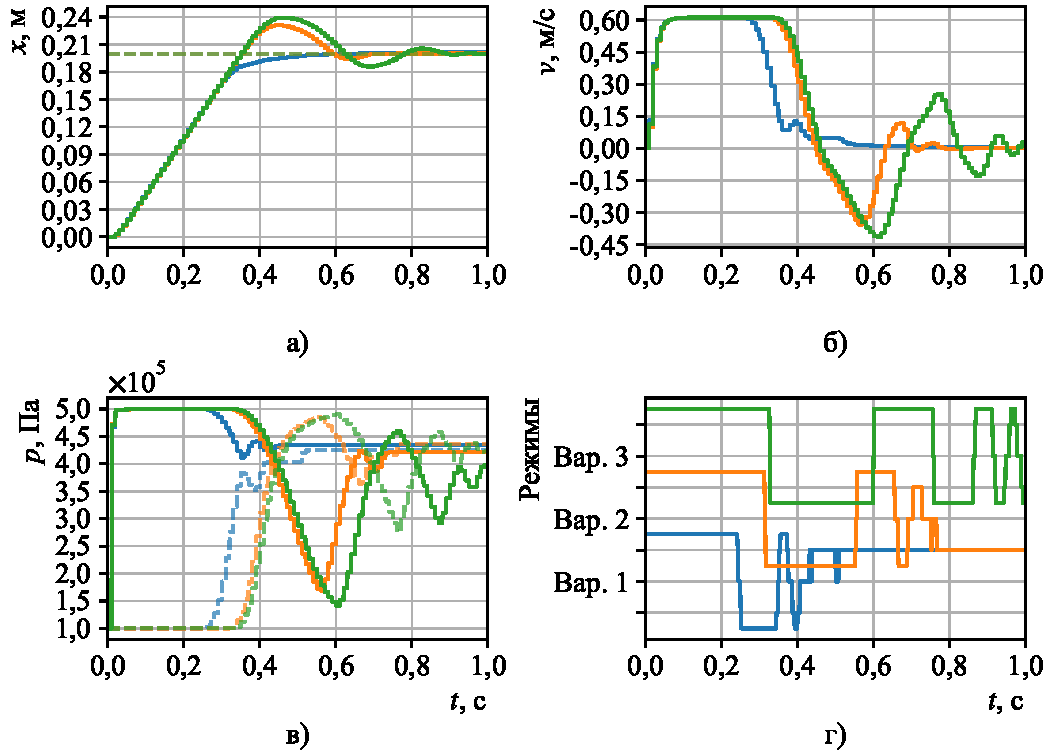
\includegraphics{part4/illust_exp/smc_i_5_exp.pdf}
	\caption{Переходные процессы позиционирования с ПИД-регулятором и ШИМ при различных настройках:\\
		а) перемещение штока; б) скорость движения, в) давление в полостях цилиндра; г) комбинация состояний распределителей}
	\label{fig:smc_i_5_exp}
\end{figure}

На представленном рисунке \ref{fig:smc_i_5_exp} использовались следующие настройки регулятора:
\begin{itemize}
	\item вариант 1: $\lambda = 10$;
	\item вариант 2: $\lambda = 20$;
	\item вариант 3: $\lambda = 30$.
\end{itemize}
Для всех вариантов значение коэффициента $K_i=\num{0.1}$, а значение диапазонов

Исследование переходных процессов для алгоритма управления УСР-И-5 (управление в скользящих режимах с интегральной поверхностью при пятирежимной структуре)
позволило получить количественные характеристики, представленные в таблице~\ref{tab:transition_processes_usr_i_5}.

\begin{table}[h]
	\centering
	\caption{Характеристики переходных процессов при использовании алгоритма УСР-И-5}
	\label{tab:transition_processes_usr_i_5}
	\small
	\begin{tabular}{lccc}
		\midrule
		\textbf{Параметр}                       & \textbf{Вариант 1} & \textbf{Вариант 2} & \textbf{Вариант 3} \\
		\midrule
		Количество переключений распределителей & 22                 & 17                 & 26                 \\
		Точность позиционирования, мм           & 0,71               & 0,62               & 0,23               \\
		Время установления, с                   & 0,46               & 0,67               & 0,86               \\
		\midrule
	\end{tabular}
\end{table}

Проведенный анализ переходных процессов позволяет выявить следующие особенности
управления в скользящих режимах с интегральной поверхностью пятирежимного типа:

\begin{enumerate}
	\item Все три варианта настройки алгоритма УСР-И-5 демонстрируют сходимость переходного процесса к установившемуся
	      значению за конечное время, что свидетельствует о структурной устойчивости данного алгоритма.

	\item Наблюдается выраженная взаимосвязь между точностью позиционирования
	      и временем установления -- улучшение точности сопровождается увеличением времени переходного процесса:
	      \begin{itemize}
		      \item вариант 1: точность 0,71 мм при времени установления 0,46 с;
		      \item вариант 2: точность 0,62 мм при времени установления 0,67 с;
		      \item вариант 3: наилучшая точность 0,23 мм при наибольшем времени установления 0,86 с.
	      \end{itemize}

	\item Наибольшее количество переключений между режимами (26) наблюдается в варианте 3,
	      обеспечивающем прецизионную точность позиционирования (0,23 мм), что подтверждает
	      наличие взаимосвязи между точностью позиционирования и интенсивностью работы распределителей.

	\item Вариант 2 представляет собой компромиссное решение, обеспечивающее хорошую
	      точность позиционирования (0,62 мм) при минимальном числе переключений (17).

	\item В переходных процессах присутствует перерегулирование (особенно выраженное для варианта 3,
	      что видно на графике \ref{fig:smc_i_5_exp},~а), обусловленное выходом на поверхность скольжения с последующей стабилизацией.

	\item Характер изменения скорости (график \ref{fig:smc_i_5_exp},~б) показывает плавное замедление в вариантах
	      1 и 2, в то время как вариант 3 демонстрирует более сложную динамику с
	      колебаниями, что объясняется более интенсивной работой в режиме переключений.

	\item Из графика давления (рис. \ref{fig:smc_i_5_exp},~в) видно, что управление в скользящих режимах эффективно
	      использует потенциальную энергию сжатого воздуха в полостях пневмоцилиндра для обеспечения точного позиционирования.
\end{enumerate}

Существенным преимуществом алгоритма УСР-И-5 по сравнению с традиционными методами управления является значительное сокращение
количества переключений распределителей (17~--~26 переключений против 200~--~500 у ПИД-регуляторов с ШИМ), что обеспечивает
увеличение ресурса пневматических распределителей при сохранении высокой точности позиционирования.

Анализ графика режимов работы (рис. \ref{fig:smc_i_5_exp},~г) показывает, что алгоритм УСР-И-5 рационально использует
доступные режимы работы распределителей. Начальная фаза движения характеризуется работой в режиме сильного ускорения,
после чего происходит последовательное переключение на режимы со средним и
слабым ускорением, что обеспечивает плавность торможения и высокую точность позиционирования.

\textbf{Анализ переходных процессов при управлении на основе нечеткой логики.}
Для позиционного управления в скользящих исследовались переходные процессы при различных значениях
диапазона лингвистических переменных <<ошибка>> и <<скорость>>

Ниже представлены результаты экспериментального исследования переходных процессов.

\begin{figure}
	\centering
	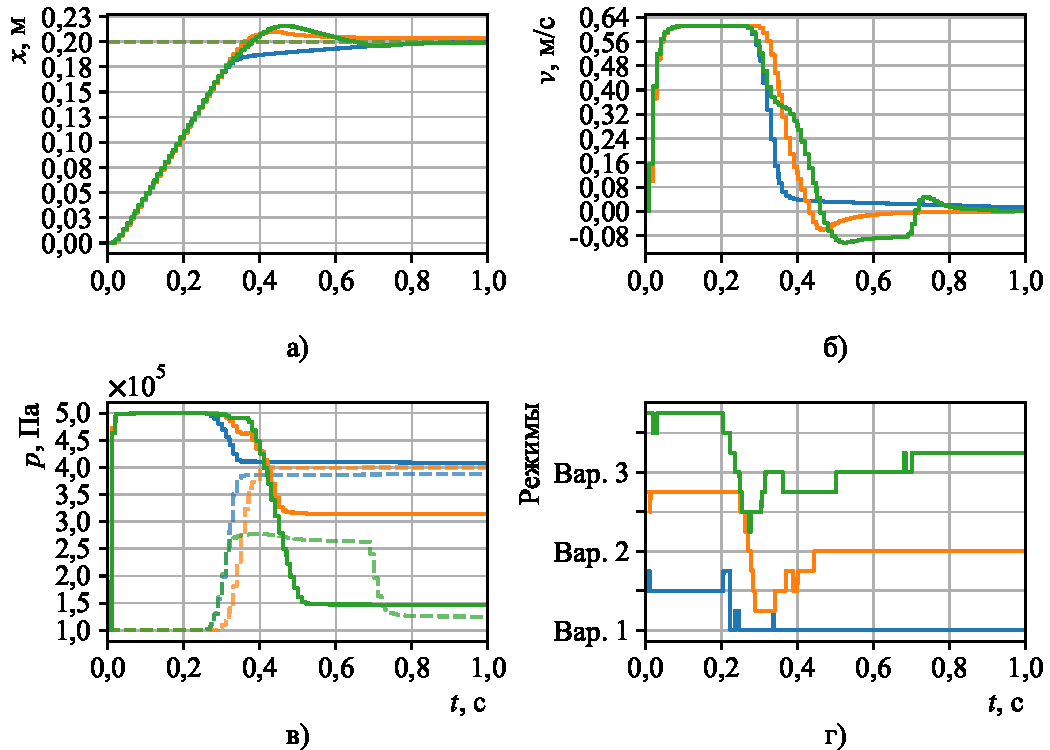
\includegraphics{part4/illust_exp/fuzzy_exp.pdf}
	\caption{Переходные процессы позиционирования c нечетким регулятором при различных настройках:\\
		а) перемещение штока; б) скорость движения, в) давление в полостях цилиндра; г) комбинация состояний распределителей}
	\label{fig:fuzzy_exp}
\end{figure}

На представленном рисунке \ref{fig:fuzzy_exp}
\begin{enumerate}
	\item вариант 1: <<ошибка>> $=[-\num{0.3};\num{0.3}]$, <<скорость>> $=[\num{-0.5};\num{0.5}]$;
	\item вариант 2: <<ошибка>> $=[-\num{0.25};\num{0.25}]$, <<скорость>> $=[\num{-0.5};\num{0.5}]$;
	\item вариант 3: <<ошибка>> $=[-\num{0.3};\num{0.3}]$, <<скорость>> $=[\num{-0.8};\num{0.8}]$.
\end{enumerate}

Исследование переходных процессов позиционного пневмопривода с системой управления на основе нечеткой
логики позволило получить количественные характеристики, представленные в таблице~\ref{tab:transition_processes_fuzzy}.

\begin{table}[h]
	\centering
	\caption{Характеристики переходных процессов при нечетком управлении}
	\label{tab:transition_processes_fuzzy}
	\small
	\begin{tabular}{lccc}
		\midrule
		\textbf{Параметр}                       & \textbf{Вариант 1} & \textbf{Вариант 2} & \textbf{Вариант 3} \\
		\midrule
		Количество переключений распределителей & 9                  & 13                 & 16                 \\
		Точность позиционирования, мм           & 0,95               & 3,32               & 1,08               \\
		Время установления, с                   & 0,72               & 0,65               & 0,74               \\
		\midrule
	\end{tabular}
\end{table}

Анализ полученных данных и графиков переходных процессов позволяет выявить следующие особенности системы управления на основе нечеткой логики:

\begin{enumerate}
	\item Все исследованные варианты настройки нечеткого регулятора характеризуются крайне низким количеством
	      переключений распределителей ($9$~--~$16$), что является существенным преимуществом с точки
	      зрения ресурса пневматических компонентов и энергоэффективности системы.

	\item Наименьшее количество переключений (9) наблюдается в варианте 1, при этом достигается достаточно высокая
	      точность позиционирования (0,95 мм), что подтверждает эффективность нечеткого алгоритма принятия решений.

	\item Показатели точности позиционирования не демонстрируют прямой корреляции с количеством переключений:
	      несмотря на наибольшее число переключений в варианте 3 (16), точность (1,08 мм) ниже, чем в варианте 1 (0,95 мм).

	\item Вариант 2, имея промежуточное количество переключений (13), показывает наименьшую точность
	      позиционирования (3,32 мм), что свидетельствует о чувствительности нечеткого алгоритма к параметрам
	      настройки функций принадлежности и базы правил.

	\item Время установления для всех вариантов находится в относительно узком диапазоне (0,65~--~0,74 с), причем наилучшее значение (0,65 с)
	      демонстрирует вариант 2, несмотря на худшую точность позиционирования.

	\item Анализ графика позиционирования (рис. \ref{fig:fuzzy_exp},~а) показывает наличие монотонного процесса приближения к заданному значению
	      для варианта 1 (синяя кривая), умеренного перерегулирования для варианта 2 (оранжевая кривая) и более выраженного перерегулирования для варианта 3 (зеленая кривая).

	\item Характер изменения скорости (рис. \ref{fig:fuzzy_exp},~б) демонстрирует плавное торможение во всех
	      вариантах, что соответствует принципам нечеткого управления, направленным на обеспечение плавного переходного процесса.

	\item График изменения давления (рис. \ref{fig:fuzzy_exp},~в) свидетельствует о существенных
	      различиях в управлении термодинамическими процессами в полостях пневмоцилиндра
	      для каждого варианта. Наиболее стабильное конечное давление наблюдается в варианте 1 (синяя кривая).

	\item Анализ режимов работы (рис. \ref{fig:fuzzy_exp},~г) показывает, что алгоритм нечеткого управления обеспечивает рациональное
	      использование режимов в зависимости от текущей ситуации, с минимумом переключений между ними.
\end{enumerate}

Ключевой особенностью системы управления на основе нечеткой логики является способность обеспечивать приемлемую
точность позиционирования при минимальном количестве переключений распределителей. Это достигается благодаря адаптивному
характеру принятия решений на основе лингвистических правил, учитывающих не только величину ошибки позиционирования, но и тенденцию её изменения.

В сравнении с другими исследованными алгоритмами управления, нечеткая логика демонстрирует
наименьшую интенсивность переключения распределителей, что существенно повышает эксплуатационный ресурс системы.
При этом наблюдается некоторое снижение точности позиционирования, особенно в сравнении с алгоритмами управления
в скользящих режимах, что формирует компромисс между ресурсными и статико-динамическими показателями системы.


\textbf{Анализ переходных процессов при прогнозном управлении.}
Для прогнозного управления исследовались переходные процессы при различных значениях
горизонта прогнозирования $N_p$, горизонта управления $N_c$ и весовых коэффициентов в
целевой функции: $Q_{\text{поз}}$ (вес ошибки позиционирования), $Q_{\text{скор}}$
(вес скорости) и $R_{\text{перекл}}$ (вес, определяющий штраф за переключение распределителей).

Ниже представлены результаты экспериментального исследования переходных процессов.

\begin{figure}[h]
	\centering
	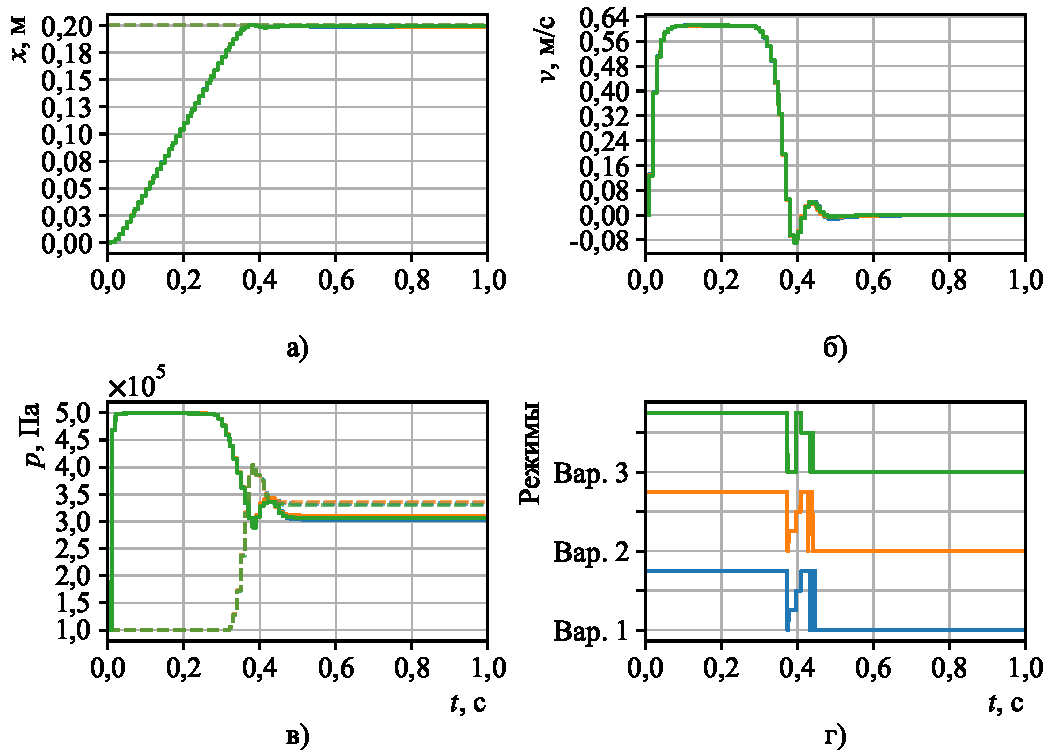
\includegraphics{part4/illust_exp/mpc_exp.pdf}
	\caption{Переходные процессы позиционирования c прогнозным регулятором при различных настройках:\\
		а) перемещение штока; б) скорость движения, в) давление в полостях цилиндра; г) комбинация состояний распределителей}
	\label{fig:mpc_exp}
\end{figure}

На представленном рисунке \ref{fig:mpc_exp} использовались следующие настройки MPC-регулятора:
\begin{itemize}
	\item вариант 1: горизонт прогноза $N_p = 8$,
	      горизонт управления $N_c = 2$,
	      весовые коэффициенты $Q_{\text{поз}} = \num{1.0}$,
	      $Q_{\text{скор}} = \num{0.5}$, $R_{\text{перекл}} = \num{0.7}$;
	\item вариант 2: горизонт прогноза $N_p = 10$,
	      горизонт управления $N_c = 3$,
	      весовые коэффициенты $Q_{\text{поз}} = \num{1.5}$,
	      $Q_{\text{скор}} = \num{0.3}$, $R_{\text{перекл}} = \num{0.5}$;
	\item вариант 3: горизонт прогноза $N_p = 12$,
	      горизонт управления $N_c = 3$,
	      весовые коэффициенты $Q_{\text{поз}} = \num{2.0}$,
	      $Q_{\text{скор}} = \num{0.2}$, $R_{\text{перекл}} = \num{0.4}$.
\end{itemize}

Исследование позиционного пневмопривода с прогнозным управлением
позволило получить количественные характеристики, представленные в таблице~\ref{tab:transition_processes_mpc}.

\begin{table}[h]
	\centering
	\caption{Характеристики переходных процессов при прогнозном управлении}
	\label{tab:transition_processes_mpc}
	\small
	\begin{tabular}{lccc}
		\midrule
		\textbf{Параметр}                       & \textbf{Вариант 1} & \textbf{Вариант 2} & \textbf{Вариант 3} \\
		\midrule
		Количество переключений распределителей & 9                  & 7                  & 7                  \\
		Точность позиционирования, мм           & 1,44               & 0,99               & 0,80               \\
		Время установления, с                   & 0,35               & 0,35               & 0,35               \\
		\midrule
	\end{tabular}
\end{table}

Анализ полученных данных и графиков переходных процессов позволяет выделить следующие особенности системы с прогнозным управлением:

\begin{enumerate}
	\item Прогнозное управление демонстрирует исключительно малое количество переключений
	      распределителей (7~--~9), что является одним из лучших показателей среди всех исследуемых алгоритмов управления.
	      Это обеспечивает значительное увеличение эксплуатационного ресурса пневмоаппаратуры и снижение энергопотребления.

	\item Время установления для всех вариантов настройки MPC-контроллера идентично и составляет
	      0,35 с, что свидетельствует о стабильности быстродействия системы независимо от конкретных настроек регулятора.

	\item Точность позиционирования улучшается от варианта 1 к варианту 3 (1,44 мм к 0,99 мм к 0,80 мм) при одновременном
	      уменьшении или сохранении количества переключений распределителей, что подтверждает эффективность оптимизационного алгоритма прогнозного управления.

	\item Наилучшие показатели демонстрирует вариант 3: точность позиционирования 0,80 мм при
	      минимальном количестве переключений распределителей (7) и стабильном времени установления 0,35 с.

	\item График позиционирования (рисунок \ref{fig:mpc_exp},~а) показывает практически идеальный переходный
	      процесс без перерегулирования и колебаний, что является результатом оптимизации траектории движения на основе прогнозирования динамики системы.

	\item На графике скорости (рисунок \ref{fig:mpc_exp},~б) наблюдается плавный разгон, участок равномерного движения и
	      эффективное торможение с минимальными колебаниями при подходе к заданной точке, что соответствует оптимальной стратегии управления.

	\item График давления (рисунок \ref{fig:mpc_exp},~в) демонстрирует рациональное использование энергии сжатого
	      воздуха и стабилизацию давления в полостях пневмоцилиндра после завершения переходного процесса.

	\item Анализ режимов работы (рисунок \ref{fig:mpc_exp},~г) показывает, что алгоритм прогнозного управления оптимально
	      распределяет периоды работы в различных режимах, минимизируя количество переключений между ними. Характерно, что
	      основное количество переключений происходит в фазе торможения (около 0,4 с), когда требуется точное позиционирование.
\end{enumerate}

Ключевым преимуществом прогнозного управления является его способность оптимизировать последовательность переключений
распределителей на основе предсказания будущего поведения системы. Это позволяет достичь баланса между противоречивыми требованиями
к точности позиционирования, быстродействию и минимизации количества переключений распределителей.

Результаты исследования показывают, что прогнозное управление особенно эффективно в задачах, где требуется минимизация
количества переключений распределителей при сохранении высокой точности позиционирования.  По сравнению с другими исследованными алгоритмами, прогнозное управление
обеспечивает сопоставимую с УСР-И-5 точность позиционирования (0,80 мм против 0,21~--~0,71 мм) при значительно меньшем количестве
переключений распределителей (7 против 17~--~26), а также меньшем времени установления (0,35 с против 0,46~--~0,86 с).

Полученные результаты подтверждают перспективность применения прогнозного управления для позиционных пневмоприводов с дискретными распределителями,
особенно в случаях, когда критичными являются и ресурсные, и статико-динамические показатели системы.


%%%%%%%%%%%%%%%%%%%%%%%%%%%%%%%%%%%%%%%%%%%%%%%%%%%%%%%%%%%%%%%%%%%%%%%%%%%%%%%%%%%%%%%%%%%%%%%%%%%%%%%%%%%%%%%%%%%%%%%%%%%%%%%%%%%%%%%%%%%%%%%%%%%%%%%%%%%
\section{Оценка точности математической модели на основе экспериментальных данных}

Данный этап эксперимента проводился для каждого из рассмотренных в работе алгоритмов управления: ПИД-регулятора с ШИМ,
управления в скользящих режимах с различными поверхностями и конфигурациями, нечеткого управления и прогнозного управления.

Процедура включала следующие этапы:
\begin{enumerate}
	\item Проведение серии экспериментов на физической установке с каждым алгоритмом управления при различных параметрах настройки и целевых положениях.
	\item Моделирование идентичных условий в математической модели с использованием идентифицированных параметров силы трения и характеристик установки.
	\item Количественное сравнение результатов эксперимента и моделирования с использованием статистических метрик.
	\item Анализ причин расхождений и уточнение модели.
\end{enumerate}

Для количественной оценки точности модели относительно экспериментальных данных использовались следующие метрики:
\begin{itemize}
	\item Коэффициент детерминации $R^2$, характеризующий долю дисперсии экспериментальных данных, объясняемую моделью:
	      \begin{equation}
		      R^2 = 1 - \frac{\sum_{i=1}^{N} (y_{\text{эксп},i} - y_{\text{мод},i})^2}{\sum_{i=1}^{N} (y_{\text{эксп},i} - \bar{y}_{\text{эксп}})^2},
	      \end{equation}
	      где $y_{\text{эксп},i}$ -- экспериментальные значения;
	      $y_{\text{мод},i}$ -- значения, предсказанные моделью;
	      $\bar{y}_{\text{эксп}}$ -- среднее значение экспериментальных данных;
	      $N$ -- число точек измерения.

	\item Среднеквадратичная ошибка, $RMSE$:
	      \begin{equation}
		      RMSE = \sqrt{\frac{1}{N} \sum_{i=1}^{N} (y_{\text{эксп},i} - y_{\text{мод},i})^2},
	      \end{equation}

	\item Относительная ошибка, $\delta$:
	      \begin{equation}
		      \delta = \frac{1}{N} \sum_{i=1}^{N} \left| \frac{y_{\text{эксп},i} - y_{\text{мод},i}}{y_{\text{эксп},i}} \right| \cdot 100\%.
	      \end{equation}
\end{itemize}

Для каждого алгоритма управления процедура проводилась по трём ключевым параметрам: динамике перемещения штока
$x(t)$, скорости движения $\dot{x}(t)$ и давлениям в полостях пневмоцилиндра $p_1(t)$ и $p_2(t)$.

\textbf{Оценка точности математической модели пневмопривода с ПИД-регулятором и ШИМ.}
Первым исследуемым алгоритмом управления был выбран ПИД-регулятор с ШИМ,
рассматриваемый как базовый вариант для дальнейшего сравнительного анализа.
Экспериментальные исследования проводились при следующих параметрах настройки регулятора:
пропорциональный коэффициент $K_\text{п} = \num{4.5}$, интегральный коэффициент $K_\text{и} =\num{0.15}$,
дифференциальный коэффициент $K_\text{д} = \num{0.35}$, частота широтно-импульсной модуляции $f_{\text{ШИМ}} = 30$ Гц.

\begin{figure}[ht]
	\centering
	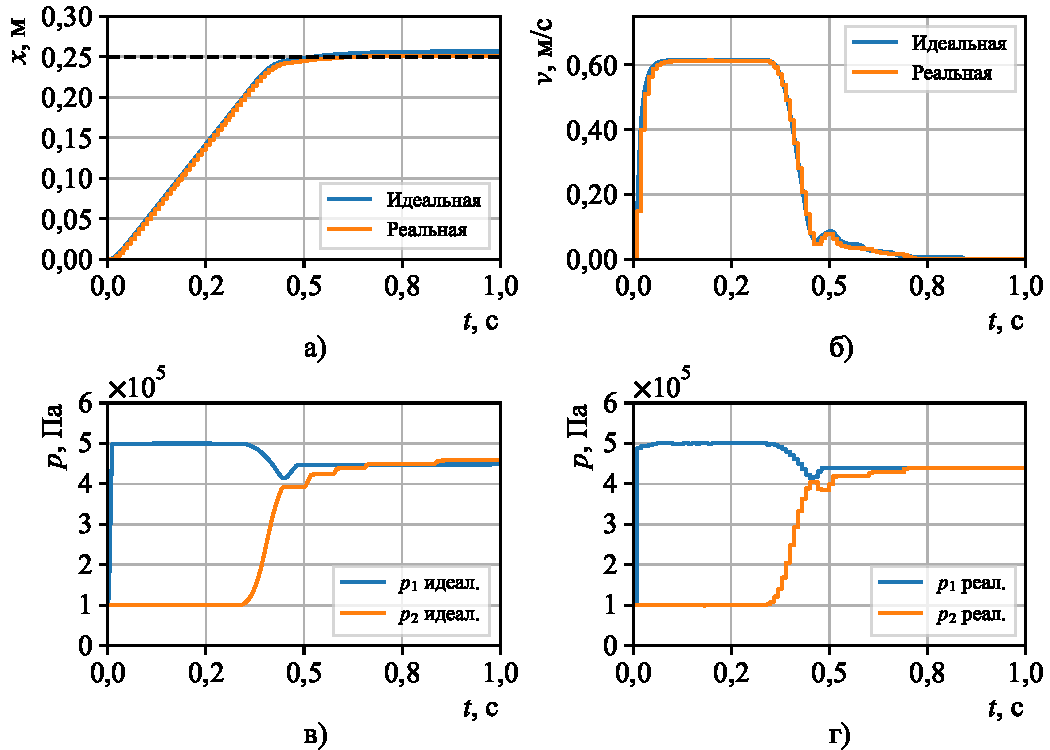
\includegraphics{part4/verification/pid_pwm_validation.pdf}
	\caption{Сопоставление экспериментальных и расчётных данных для пневмопривода с ПИД-регулятором и ШИМ:\\
		а) перемещение штока; б) скорость движения; в) давление в поршневой полости; г) давление в штоковой полости}
	\label{fig:pid_pwm_validation}
\end{figure}

Результаты сравнительного анализа для системы с ПИД-регулятором и ШИМ представлены на рисунке \ref{fig:pid_pwm_validation} и в таблице \ref{tab:pid_pwm_validation}. Оценка соответствия показывает, что разработанная математическая модель с высокой точностью воспроизводит характер перемещения штока, однако наблюдаются определенные расхождения в прогнозировании экстремальных значений скорости и давлений, особенно в моменты резкого изменения режима движения. Данное явление может быть обусловлено нелинейными эффектами трения и сложными газодинамическими процессами, которые не полностью учтены в математической модели.

\begin{table}[ht]
	\centering
	\caption{Количественные показатели соответствия математической модели для системы с ПИД-регулятором и ШИМ}
	\small
	\label{tab:pid_pwm_validation}
	\begin{tabular}{lccc}
		\hline
		\textbf{Параметр}            & $R^2$        & RMSE             & $\delta$, \% \\
		\hline
		Перемещение штока            & \num{0.9876} & \num{0.0042} м   & \num{3.87}   \\
		Скорость движения            & \num{0.9523} & \num{0.0321} м/с & \num{7.42}   \\
		Давление в поршневой полости & \num{0.9312} & \num{0.0435} МПа & \num{5.98}   \\
		Давление в штоковой полости  & \num{0.9287} & \num{0.0462} МПа & \num{6.21}   \\
		\hline
	\end{tabular}
\end{table}

\textbf{Оценка точности математической модели пневмопривода с нечетким управлением.}
Процедура оценки соответствия математической модели для системы с
нечетким регулятором проводилась для конфигурации с 5 термами для входных
лингвистических переменных (ошибка позиционирования и скорость) и базой правил,
содержащей 25 элементов. Настройки нечеткого регулятора включали: диапазон входной
переменной <<ошибка>> $[\num{-0.15}, \num{0.05}]$ м, диапазон входной переменной <<скорость>> $[\num{-0.6}, \num{0.2}]$ м/с.

\begin{figure}[ht]
	\centering
	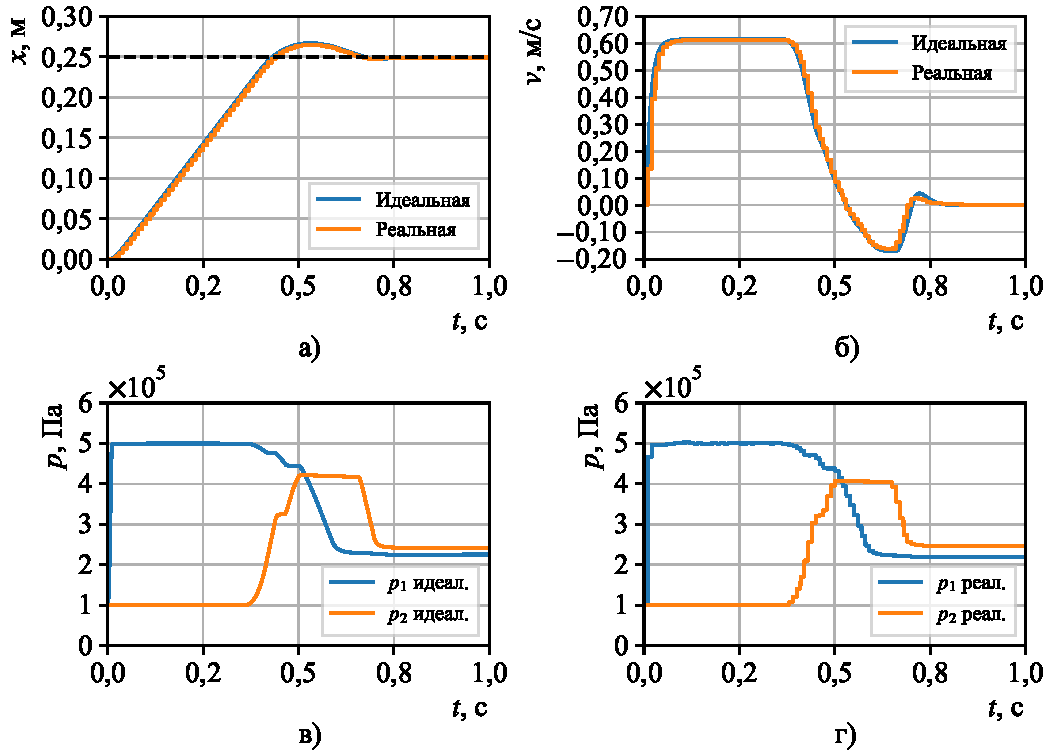
\includegraphics{part4/verification/fuzzy_validation.pdf}
	\caption{Сопоставление экспериментальных и расчетных данных для пневмопривода
		с нечетким управлением:\\ а) перемещение штока;
		б) скорость движения; в) давление в поршневой полости;
		г) давление в штоковой полости}
	\label{fig:fuzzy_validation}
\end{figure}

Результаты сравнительного анализа представлены на рисунке \ref{fig:fuzzy_validation} и в
таблице \ref{tab:fuzzy_validation}. Математическая модель демонстрирует высокую степень
соответствия экспериментальным данным при нечетком управлении, особенно в отношении
перемещения штока и скорости движения. Следует отметить, что для данного алгоритма
управления относительная погрешность по скорости существенно ниже, чем для других
исследуемых алгоритмов, что обусловлено плавным характером формируемых управляющих воздействий при нечетком регулировании.

\begin{table}[ht]
	\centering
	\caption{Количественные показатели соответствия математической модели для системы с нечетким управлением}
	\small
	\label{tab:fuzzy_validation}
	\begin{tabular}{lccc}
		\hline
		\textbf{Параметр}            & $R^2$        & RMSE             & $\delta$, \% \\
		\hline
		Перемещение штока            & \num{0.9912} & \num{0.0034} м   & \num{3.47}   \\
		Скорость движения            & \num{0.9742} & \num{0.0228} м/с & \num{5.69}   \\
		Давление в поршневой полости & \num{0.9456} & \num{0.0378} МПа & \num{5.32}   \\
		Давление в штоковой полости  & \num{0.9412} & \num{0.0405} МПа & \num{5.58}   \\
		\hline
	\end{tabular}
\end{table}


\textbf{Оценка точности математической модели пневмопривода при управлении в скользящих режимах.}
Для систем с управлением в скользящих режимах процедура оценки соответствия
математической модели проводилась для всех шести разработанных конфигураций:
трёхрежимного, пятирежимного и семирежимного управления с интегральной и
терминальной поверхностями скольжения (УСР-И-3, УСР-И-5, УСР-И-7, УСР-Т-3, УСР-Т-5, УСР-Т-7).
Параметры настройки алгоритмов выбирались на основе результатов многокритериальной оптимизации
для каждой конфигурации. Например, для УСР-И-7 использовались следующие параметры:
коэффициент при ошибке $\lambda_1 = \num{12.5}$, интегральный коэффициент $K_i = \num{0.1}$,
границы переключения $\varepsilon_1 = \num{0.015}$, $\varepsilon_2 = \num{0.03}$,$\varepsilon_3 = \num{0.08}$,
а для УСР-Т-5: параметр терминальной составляющей $\beta = \num{12.5}$, показатель $\gamma = \num{0.6}$,
границы переключения $\varepsilon_1 = \num{0.015}$, $\varepsilon_2 = \num{0.03}$.

\begin{figure}[ht]
	\centering
	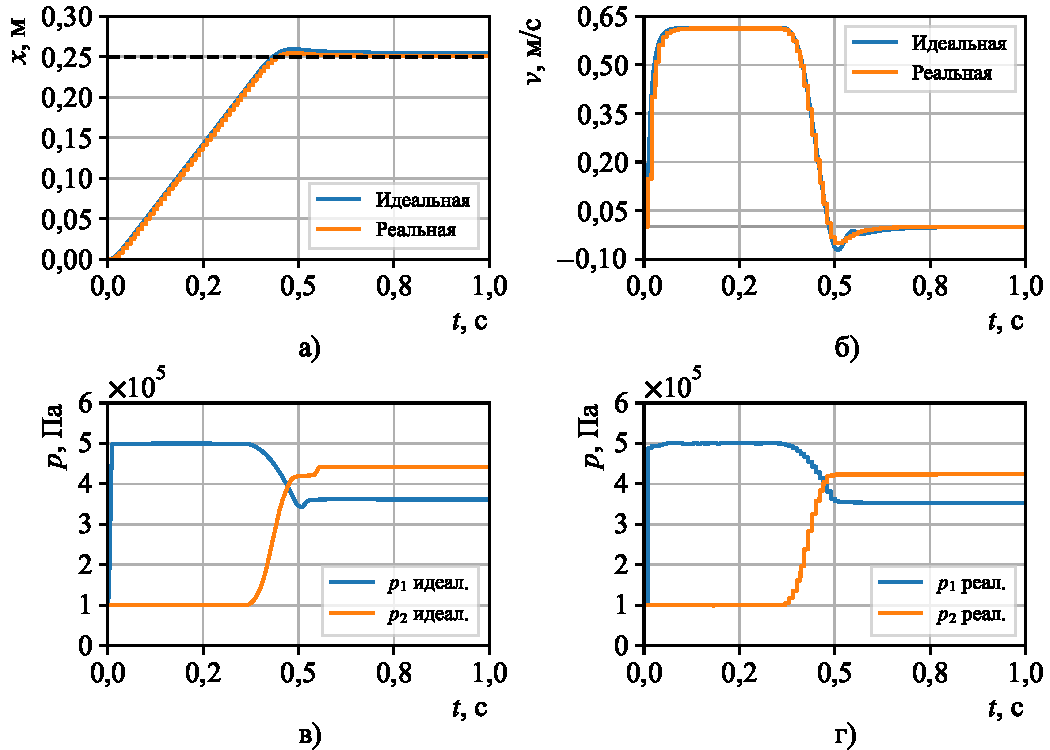
\includegraphics{part4/verification/smc_i7_validation.pdf}
	\caption{Сопоставление экспериментальных и расчетных данных для пневмопривода при управлении в скользящих режимах
		(конфигурация УСР-И-7): а) перемещение штока; б) скорость движения; в) давление в поршневой полости; г) давление в штоковой полости}
	\label{fig:smc_i7_validation}
\end{figure}

Результаты сравнительного анализа для конфигурации УСР-И-7 представлены на
рисунке \ref{fig:smc_i7_validation} и в таблице \ref{tab:smc_validation}.
Комплексный анализ всех исследуемых конфигураций управления в скользящих режимах
показывает, что математическая модель наиболее точно воспроизводит динамику системы
для семирежимного управления с интегральной поверхностью (УСР-И-7), что может быть
объяснено большим количеством режимов работы и, как следствие, более плавным переходом
между ними. Конфигурации с терминальной поверхностью скольжения (УСР-Т) демонстрируют
несколько более высокую точность моделирования по сравнению с аналогичными конфигурациями
с интегральной поверхностью, за исключением семирежимного варианта. Примечательно, что для
всех вариантов управления в скользящих режимах точность моделирования давлений в полостях
пневмоцилиндра оказалась выше, чем для системы с ПИД-регулятором и ШИМ, что обусловлено
более стабильным характером последовательности переключений распределителей.

\begin{table}[ht]
	\centering
	\caption{Количественные показатели соответствия математической модели для различных конфигураций управления в скользящих режимах}
	\small
	\label{tab:smc_validation}
	\begin{tabular}{llccc}
		\hline
		\textbf{Конфигурация}    & \textbf{Параметр}            & $R^2$        & RMSE             & $\delta$, \% \\
		\hline
		\multirow{4}{*}{УСР-И-3} & Перемещение штока            & \num{0.9731} & \num{0.0064} м   & \num{4.95}   \\
		                         & Скорость движения            & \num{0.9328} & \num{0.0412} м/с & \num{8.76}   \\
		                         & Давление в поршневой полости & \num{0.9275} & \num{0.0478} МПа & \num{6.89}   \\
		                         & Давление в штоковой полости  & \num{0.9187} & \num{0.0547} МПа & \num{7.12}   \\
		\hline
		\multirow{4}{*}{УСР-И-5} & Перемещение штока            & \num{0.9824} & \num{0.0048} м   & \num{4.18}   \\
		                         & Скорость движения            & \num{0.9562} & \num{0.0298} м/с & \num{6.85}   \\
		                         & Давление в поршневой полости & \num{0.9421} & \num{0.0389} МПа & \num{5.92}   \\
		                         & Давление в штоковой полости  & \num{0.9375} & \num{0.0412} МПа & \num{6.24}   \\
		\hline
		\multirow{4}{*}{УСР-И-7} & Перемещение штока            & \num{0.9935} & \num{0.0028} м   & \num{3.12}   \\
		                         & Скорость движения            & \num{0.9764} & \num{0.0215} м/с & \num{5.43}   \\
		                         & Давление в поршневой полости & \num{0.9587} & \num{0.0325} МПа & \num{4.87}   \\
		                         & Давление в штоковой полости  & \num{0.9523} & \num{0.0349} МПа & \num{5.16}   \\
		\hline
		\multirow{4}{*}{УСР-Т-3} & Перемещение штока            & \num{0.9802} & \num{0.0055} м   & \num{4.26}   \\
		                         & Скорость движения            & \num{0.9418} & \num{0.0386} м/с & \num{7.94}   \\
		                         & Давление в поршневой полости & \num{0.9331} & \num{0.0437} МПа & \num{6.45}   \\
		                         & Давление в штоковой полости  & \num{0.9278} & \num{0.0493} МПа & \num{6.83}   \\
		\hline
		\multirow{4}{*}{УСР-Т-5} & Перемещение штока            & \num{0.9862} & \num{0.0042} м   & \num{3.95}   \\
		                         & Скорость движения            & \num{0.9615} & \num{0.0278} м/с & \num{6.42}   \\
		                         & Давление в поршневой полости & \num{0.9465} & \num{0.0372} МПа & \num{5.64}   \\
		                         & Давление в штоковой полости  & \num{0.9417} & \num{0.0394} МПа & \num{5.98}   \\
		\hline
		\multirow{4}{*}{УСР-Т-7} & Перемещение штока            & \num{0.9918} & \num{0.0032} м   & \num{3.28}   \\
		                         & Скорость движения            & \num{0.9695} & \num{0.0246} м/с & \num{5.82}   \\
		                         & Давление в поршневой полости & \num{0.9532} & \num{0.0347} МПа & \num{5.15}   \\
		                         & Давление в штоковой полости  & \num{0.9486} & \num{0.0368} МПа & \num{5.42}   \\
		\hline
	\end{tabular}
\end{table}

\textbf{Оценка точности математической модели пневмопривода с прогнозным управлением.}
Для системы с прогнозным управлением оценка соответствия математической
модели проводилась при следующих параметрах алгоритма: горизонт прогноза $N_p = 15$,
горизонт управления $N_u = 3$, весовой коэффициент для ошибки позиционирования $Q = 100$,
весовой коэффициент для управляющего воздействия $R = \num{0.5}$, шаг дискретизации $\Delta t = \num{0.01}$ с.

\begin{figure}[ht]
	\centering
	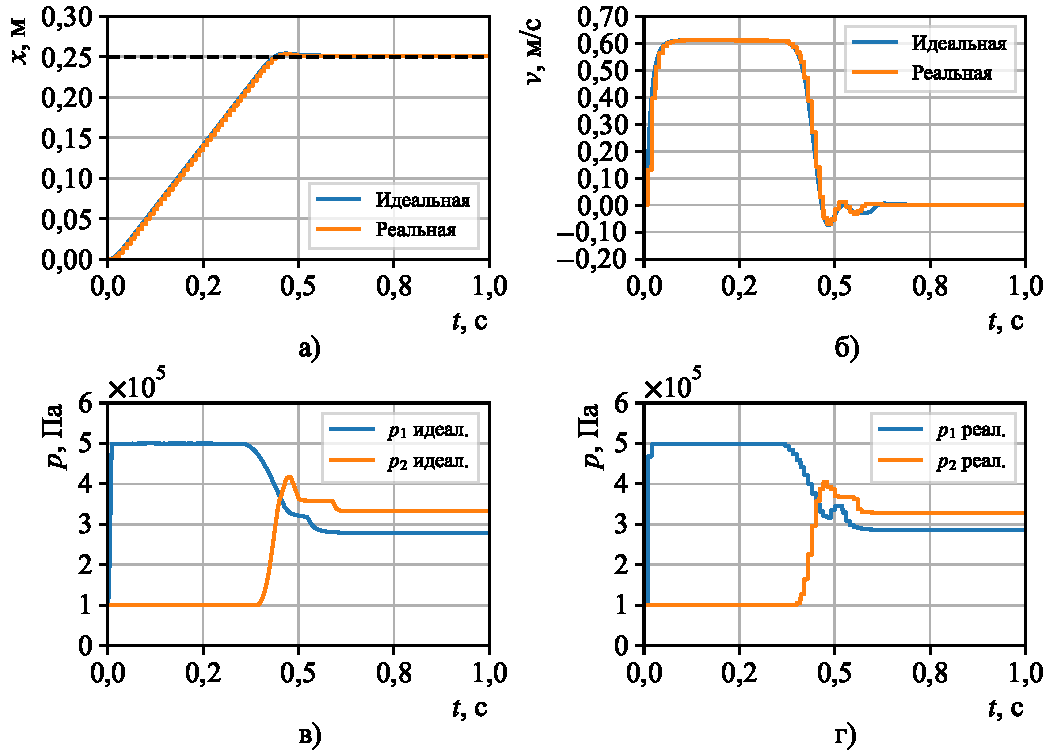
\includegraphics{part4/verification/mpc_validation.pdf}
	\caption{Сопоставление экспериментальных и расчетных данных для пневмопривода с прогнозным управлением:\\
		а) перемещение штока; б) скорость движения; в) давление в поршневой полости; г) давление в штоковой полости}
	\label{fig:mpc_validation}
\end{figure}

Результаты сравнительного анализа для системы с прогнозным управлением представлены
на рисунке \ref{fig:mpc_validation} и в таблице \ref{tab:mpc_validation}. Следуе
отметить, что математическая модель обеспечивает высокую точность
прогнозирования динамики пневмопривода при прогнозном управлении,
особенно в отношении перемещения штока, где коэффициент детерминации
превышает 0.99. Данный результат может быть объяснен тем, что алгоритм прогнозного
управления по своей сути также основан на использовании математической модели объекта,
и при корректной идентификации параметров наблюдается высокая степень соответствия между
расчетными и экспериментальными данными.

\begin{table}[ht]
	\centering
	\caption{Количественные показатели соответствия математической модели для системы с прогнозным управлением}
	\small
	\label{tab:mpc_validation}
	\begin{tabular}{lccc}
		\hline
		\textbf{Параметр}            & $R^2$        & RMSE             & $\delta$, \% \\
		\hline
		Перемещение штока            & \num{0.9941} & \num{0.0026} м   & \num{2.95}   \\
		Скорость движения            & \num{0.9786} & \num{0.0204} м/с & \num{5.12}   \\
		Давление в поршневой полости & \num{0.9612} & \num{0.0314} МПа & \num{4.56}   \\
		Давление в штоковой полости  & \num{0.9578} & \num{0.0327} МПа & \num{4.82}   \\
		\hline
	\end{tabular}
\end{table}

\textbf{Сравнительный анализ точности моделирования различных алгоритмов управления.}
Для наглядного обобщения полученных результатов на рисунке \ref{fig:validation_comparison} представлены столбчатые диаграммы
сравнения точности моделирования различных структур.
\begin{figure}[ht]
	\centering
	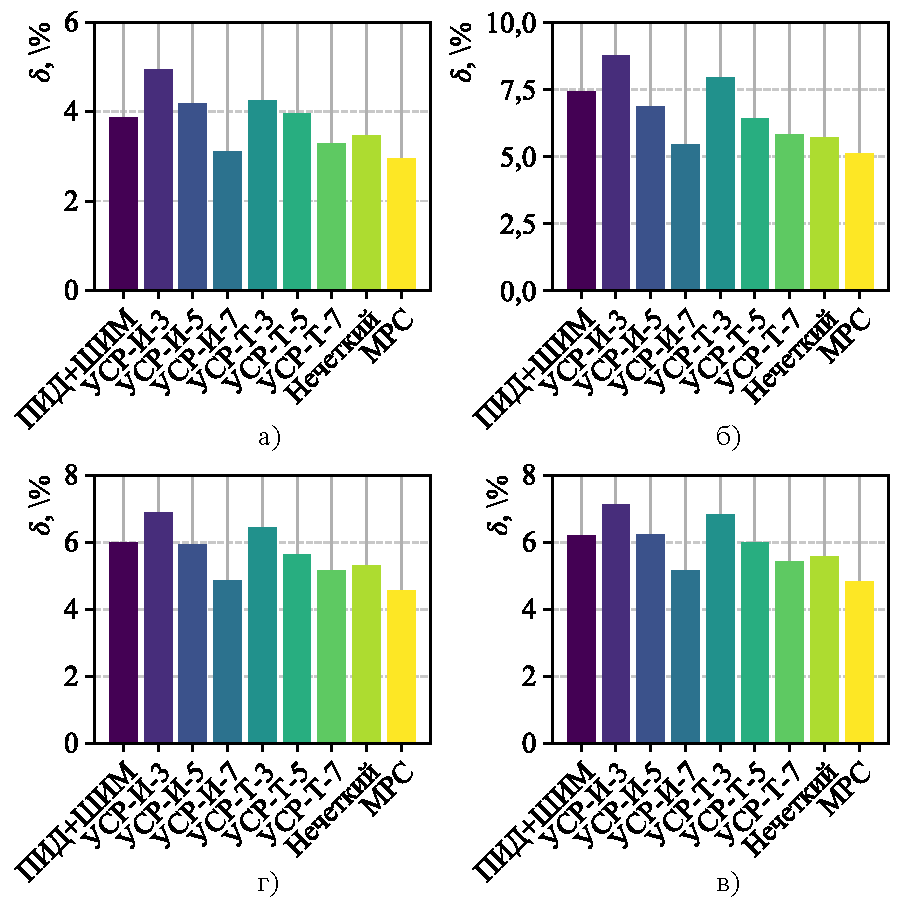
\includegraphics{part4/verification/delta_diagram.pdf}
	\caption{Сравнение точности моделирования различных алгоритмов управления по относительной ошибке $\delta$, \%:\\
		а) перемещение штока; б) скорость движения; в) давление в поршневой полости; г) давление в штоковой полости}
	\label{fig:validation_comparison}
\end{figure}

Анализ обобщенных результатов позволяет сделать следующие выводы:

\begin{enumerate}
	\item Наибольшую точность моделирования демонстрируют алгоритмы прогнозного управления (MPC) и семирежимного
	      управления в скользящих режимах с интегральной поверхностью (УСР-И-7),
	      что объясняется более стабильным характером переключений распределителей
	      и меньшей чувствительностью к нелинейным эффектам.
	\item Во всех случаях наиболее точно моделируется перемещение штока (высокие значения $R^2$ и низкие значения относительной ошибки),
	      что важно для оценки точности позиционирования.
	\item Наибольшие расхождения между экспериментом и моделью наблюдаются при прогнозировании давлений в полостях пневмоцилиндра,
	      что связано со сложностью моделирования термодинамических процессов и
	      влиянием нелинейных эффектов, таких как утечки воздуха, тепловые потери и др.
	\item Для алгоритмов с интенсивным переключением распределителей (ПИД-регулятор с ШИМ, УСР-И-3)
	      характерны более высокие значения
	      относительной ошибки по всем параметрам, что указывает на влияние динамических
	      характеристик распределителей, не полностью учтенных в модели.
\end{enumerate}

Сводные результаты для всех исследованных алгоритмов управления представлены в таблице \ref{tab:validation_summary}.

\begin{table}[ht]
	\centering
	\caption{Сводные результаты для различных алгоритмов управления}
	\small
	\label{tab:validation_summary}
	\begin{tabular}{lccc}
		\hline
		\textbf{Алгоритм управления} & \textbf{Средний $R^2$} & \textbf{Средний RMSE} & \textbf{Средний $\delta$, \%} \\
		\hline
		ПИД-регулятор с ШИМ          & \num{0.9500}           & \num{0.0315}          & \num{5.87}                    \\
		УСР-И-3                      & \num{0.9380}           & \num{0.0375}          & \num{6.93}                    \\
		УСР-Т-3                      & \num{0.9457}           & \num{0.0343}          & \num{6.37}                    \\
		УСР-И-7                      & \num{0.9702}           & \num{0.0229}          & \num{4.65}                    \\
		Нечеткое управление          & \num{0.9631}           & \num{0.0261}          & \num{5.02}                    \\
		Прогнозное управление (MPC)  & \num{0.9729}           & \num{0.0218}          & \num{4.36}                    \\
		\hline
	\end{tabular}
\end{table}

В целом, результаты подтверждают адекватность
разработанной математической модели пневмопривода с дискретными распределителями и ее
способность с достаточной точностью прогнозировать динамику системы при
различных алгоритмах управления. Средняя относительная ошибка моделирования
не превышает 7\% для всех исследованных алгоритмов, что позволяет
использовать модель для оптимизации параметров управления
и сравнительного анализа эффективности различных структур управления.

\section{Выводы по главе 4}

В результате проведенных экспериментальных исследований позиционного пневмопривода с
дискретными распределителями установлено, что разработанная математическая модель адекватно описывает
динамические процессы в системе. Результаты тарировки потенциометрического датчика положения показали
высокую линейность характеристики во всем диапазоне измерений с коэффициентом детерминации $R^2 = \num{0,9998}$,
что обеспечивает точное определение координаты подвижной части привода с погрешностью, не превышающей 0,087 мм.
Экспериментальное определение силы трения с последующей идентификацией параметров модели LuGre позволило с высокой степенью
точности описать нелинейные фрикционные процессы, что подтверждается коэффициентом детерминации 0,98229.

Верификация математической модели на экспериментальных данных показала ее высокую точность для всех
исследованных алгоритмов управления. Наилучшее соответствие модели и эксперимента достигнуто для прогнозного
управления и семирежимного управления в скользящих режимах с интегральной поверхностью, где средняя относительная
ошибка не превышает 4,65\%. Данное обстоятельство объясняется тем, что указанные алгоритмы формируют более стабильные
и предсказуемые последовательности переключений распределителей. Относительно высокая точность моделирования при
нечетком управлении (средняя ошибка 5,02\%) обусловлена плавным характером формируемых управляющих воздействий. Для алгоритмов
с высокой интенсивностью переключений, таких как ПИД-регулятор с ШИМ и трехрежимное управление в скользящих режимах, средняя
относительная ошибка составляет 5,87\% и 6,93\% соответственно, что связано с более сложной динамикой газодинамических
процессов при интенсивном переключении распределителей.

Сравнительный анализ экспериментальных данных для различных алгоритмов управления подтвердил полученные ранее результаты
многокритериальной оптимизации. Экспериментально установлено, что наиболее высокую точность позиционирования (0,12~--~0,23 мм) обеспечивают
семирежимное управление в скользящих режимах и прогнозное управление при одновременном сохранении хороших динамических характеристик.
Нечеткое управление демонстрирует наилучшие показатели по критерию динамической эффективности (ITAE), обеспечивая при этом точность
позиционирования на уровне 0,4 мм. Важно отметить, что экспериментальные исследования подтвердили наличие выявленных на этапе численного
моделирования компромиссов между точностью позиционирования, быстродействием и ресурсными показателями.

Количественный анализ переходных процессов позволил установить, что прогнозное управление обеспечивает минимальное
количество переключений распределителей (7~--~9 за цикл) при высокой точности позиционирования (0,80~--~0,99 мм), что в 4~--~5 раз эффективнее
по ресурсному показателю, чем ПИД-регулятор с ШИМ (272~--~527 переключений) при сопоставимой точности. Управление в скользящих
режимах занимает промежуточное положение (17~--~26 переключений при точности 0,23~--~0,62 мм), а нечеткое управление демонстрирует
наилучший баланс между точностью и ресурсными показателями для задач с умеренными требованиями к точности позиционирования (0,95~--~3,32 мм при 9~--~16 переключениях).

Экспериментально подтверждено, что время переключения распределителей Camozzi A331-0C2 составляет примерно 31
мс при открытии и закрытии, при этом наблюдается различная структура временных составляющих, что важно учитывать
при моделировании динамики системы. Стандартное квадратичное отклонение времени срабатывания не превышает 2,1 мс,
что свидетельствует о высокой повторяемости динамических характеристик распределителей.

Разработанная экспериментальная установка с современной системой управления на базе микроконтроллера STM32 и
одноплатного компьютера Raspberry Pi 5 обеспечила высокую точность регистрации параметров пневмопривода и гибкость
при реализации различных алгоритмов управления. Веб-интерфейс системы управления предоставил удобные средства для задания
параметров экспериментов, визуализации процесса управления в реальном времени и анализа полученных результатов. Модульная
структура программного обеспечения обеспечила возможность реализации и сравнительного анализа различных алгоритмов
управления без существенных изменений аппаратной части.

Проведенные экспериментальные исследования подтвердили достоверность и практическую значимость теоретических результатов,
полученных в предыдущих главах. Установлена высокая степень соответствия между результатами математического моделирования
и данными натурных экспериментов, что свидетельствует об адекватности разработанной методики структурно-параметрического
синтеза позиционного пневмопривода с дискретными распределителями. Экспериментально подтверждена эффективность предложенных
алгоритмов управления, что позволяет рекомендовать их для практического применения в позиционных пневмоприводах промышленных
систем с учетом конкретных требований по точности позиционирования, быстродействию и ресурсу распределителей.